% adapted by WS from SSR's Word document and from the 5-part series at
% https://www.overleaf.com/learn/latex/How_to_Write_a_Thesis_in_LaTeX_(Part_1):_Basic_Structure
% reviewed by MAM
\documentclass[12pt,twosided]{report}
\usepackage[titletoc]{appendix} % for adding appendix to TOC
\usepackage{biblatex}  % reference management
\usepackage{geometry}  % better margins and margin control
\usepackage{graphicx}  % to include figures

\usepackage{hyperref}  % internal and external links
\usepackage[utf8]{inputenc}  % support for non-ASCII characters
\usepackage{listings}  % typset code
\usepackage{outlines}  % easy nesting of lists
\usepackage{tabularx}  % more control over table column width
\usepackage{titlesec}  % customize chapter title 
\usepackage{upquote}  % prevent mishandling of single quotes in listings
\usepackage{pythontex}
\usepackage{setspace}

% TODO: Customize the appearance of hyperref links using \hypersetup
% See https://en.wikibooks.org/wiki/LaTeX/Hyperlinks#Customization

% Custom format of chapter title.
\titleformat{\chapter}[hang]{\bf\huge}{\thechapter.}{2pc}{}

% Separate folder for images named 'images'.
\graphicspath{ {images/} }

% Separate file for references
\addbibresource{references.bib}

% Replace with your title
\title{Chhoti Si Kaavish}

% Allow recalling document title
% from https://tex.stackexchange.com/a/15806/44301
\makeatletter\let\Title\@title\makeatother  

\begin{document}


% Python environment
\lstnewenvironment{python}[1][]
{
\pythonstyle
\lstset{#1}
}
{}

% Python for external files
\newcommand\pythonexternal[2][]{{
\pythonstyle
\lstinputlisting[#1]{#2}}}

% Python for inline
\newcommand\pythoninline[1]{{\pythonstyle\lstinline!#1!}}


%% Define your thesis title, your name, your school, and your month and year of graduation here
\newcommand{\reportTitle}{InstaWeight}
\newcommand{\yourNameA}{Atif Mehmood}
\newcommand{\yourNameB}{Sayyda Sahar Fatima}
\newcommand{\yourNameC}{Mohammad Ateeb Ahmed}

\newcommand{\yourSchool}{Dhanani School of Science and Engineering}
\newcommand{\yourMonth}{Spring}
\newcommand{\yourYear}{2020}

%%%%%%%%%%%%%%%%%%%%%%%%%%%%%%%%%%%%%%%%%%%%%%%%%%%%%%%%%
% Do not edit these lines unless you wish to customize
% the template
%%%%%%%%%%%%%%%%%%%%%%%%%%%%%%%%%%%%%%%%%%%%%%%%%%%%%%%%%



\begin{titlepage}
%%%%%%%%%%%%%%%%
%% First Title Page
%%%%%%%%%%%%%%%%
\begin{center}
	%\color{goldenrod}
    \vspace*{1cm}
    
\includegraphics[width=0.25\textwidth]{images/GoldenLogo.png}\\
 	\vspace*{3cm}
    \large
    \textbf{\MakeUppercase{\reportTitle}}\\
 	\vspace{2cm}
 	\normalsize
 	\ifdefined\yourNameE
 	    \textbf{\yourNameA\\ \yourNameB\\ \yourNameC\\ \yourNameD\\ \yourNameE}
 	\else
 	    \ifdefined\yourNameD
 	        \textbf{\yourNameA\\ \yourNameB\\ \yourNameC\\ \yourNameD}
 	    \else
 	        \ifdefined\yourNameC
 	            \textbf{\yourNameA\\ \yourNameB\\ \yourNameC}
 	        \else
 	            \ifdefined\yourNameB
 	                \textbf{\yourNameA\\ \yourNameB}
 	            \else
 	                \textbf{\yourNameA\\}
 	            \fi
 	        \fi 
 	     \fi
 	\fi 	
	\vfill

 	%\vspace*{cm}
    \small\textbf{HABIB UNIVERSITY \\ KARACHI, PAKISTAN\\ 2020}

\end{center}
\clearpage
%%%%%%%%%%%%%%%%
%% Second Title Page
%%%%%%%%%%%%%%%%
\begin{center}
\begin{singlespacing}
\textbf{\MakeUppercase{\reportTitle}}\\
\vspace{10\baselineskip}
The Kaavish Report\\
presented to the academic faculty\\
\vspace{2\baselineskip}
by\\
\vspace{2\baselineskip}
\yourNameA\\
\ifdefined\yourNameB
	\vspace{1\baselineskip}
	\yourNameB\\
\fi
\ifdefined\yourNameC
	\vspace{1\baselineskip}
	\yourNameC\\
\fi
\ifdefined\yourNameD
	\vspace{1\baselineskip}
	\yourNameD\\
\fi
\ifdefined\yourNameE
	\vspace{1\baselineskip}
	\yourNameE\\
\fi
\vspace{1.5\baselineskip}
in partial fulfillment
of the requirements for \\
\textit{Bachelor of Science} \\ 
Computer Science \\
\yourSchool\\
\vspace{2\baselineskip}
Habib University\\
\yourMonth{} \yourYear{}\\
\vspace{1\baselineskip}
Copyright \copyright{} \yourYear{} Habib University

\end{singlespacing}
\end{center}

\end{titlepage}

  % title page
 \thispagestyle{empty}
\centerline{\textbf{\LARGE InstaWeight}}
\vfill

This Kaavish project was supervised by:\\\bigskip\\\bigskip\\\bigskip

% TODO: Use the appropriate table below depending on whether you have an external advisor. Comment out the unused table.

% If no external supervisor.
\hfill %
\begin{tabular}{l}
    
  \line(1,0){200} \\
   Dr. Akhlaque Ahmed
 \\ % Name of your CS supervisor
  Faculty of Computer Science\\
  Habib University
\end{tabular}\\\bigskip\bigskip

% % If external supervisor.
% \begin{tabularx}{\linewidth}{lXl}
%   \line(1,0){175} & & \line(1,0){175}\\  % Signatures.
%   My External Supervisor & & My Internal Supervisor \\ % Names of your supervisors
%   Designation & & Faculty of Computer Science\\  % External supervisor's role/job tile at their company.
%   Awesome Ltd. & & Habib University  % External supervisor's company.
% \end{tabularx}\\\bigskip\bigskip

Approved by the Faculty of Computer Science on \hrulefill.

%%% Local Variables:
%%% mode: latex
%%% TeX-master: "report"
%%% End:
  % approval page.

\newpage

\vspace*{\fill} 
\begin{quote} 

\begin{center}
    ``Your sickness is from you, but you do not perceive it and your remedy is within you, but you do not sense it. You presume you are a small entity, but within you is enfolded the entire Universe. You are indeed the evident book, by whose alphabets the hidden becomes manifest. Therefore, you have no need to look beyond yourself. What you seek is within you, if only you reflect." (Imam Ali A.S)
\end{center}
    
    
\end{quote}
\vspace*{\fill}


\chapter*{}
\vspace*{\fill}
\begin{center}
    This project is dedicated to our beloved parents, respectable professors and supportive friends We pray to Allah Almighty for their health and pray to keep them saved from this Covid-19 and all other diseases. 
\end{center}

\vspace*{\fill}

\chapter*{Acknowledgements}
\
By the grace of Allah Almighty this journey comes to its end. It was not possible without the sincere, cooperative, and brilliant people around us. We would like to give credit of our success to several individuals and of course to ``Habib University''. Firstly, we would like to express our sincere thanks to our supervisor, professor ``Dr Akhlaque Ahmed'' who supported us through out the project. His valuable advises, insightful comments, helpful information, and unceasing ideas, even in this pandemic and uncertain situation of COVID-19, helped us to successfully complete our project. It wasn't possible without his relentless help.  \newline
We also wish to express our sincere thanks to all our professors  and``Kaavish Working Group'', who guided us through out our journey, keep us updated in this worst time and answered every query on time. Furthermore, we would like appreciate the guidance given by other supervisors as well as the panel (Dr. Taj, Dr. Abdul Samad, Dr Umair Azfar and Miss Nadia Nasir) especially in our project presentation, who gave valuable comments and advises that improved our presentation skills. \newline
We would also like to say thanks to Folio3 Software Inc, who gave their precious time to serve us and supervised us through out the project. We are really thankful to them to provide us Real Sense Depth Camera to capture depth images and dataset. \newline
We are also thankful to our parents who support us and stand by us through the peaks and valleys of life. \newline
Last but not least, we are also thankful to all our sincere friends who helped us to cheer up the mood and gave us moral support in bad times and special thanks to Syed Muhammad Hasan who helped us in dataset collection and annotation, Aniqa Ahsan and Ateeb Ahmed who also helped us in dataset annotation. 
\chapter*{Abstract}
The project, ``instaWeight" aims to automate the process of weight estimation using machine learning and deep learning techniques. It makes the whole process of weight estimation and then tracking the history of cattle's weight in a large farm or in live stock business automatic. It calculates the cattle's weight and then maintain the history of it through admin panel, which keeps all the records saved for years. 
\newline
This report gives the complete insight of the project and enlightens each idea in detail. It first describes the problem in the manual way of weight estimation then provides the solution, proposed by ``Team - instaWeight". It also gives a detailed literature review to get the idea of other similar work done in the same domain. The report also have separate sections on software requirement specification and software design specification, which provides the insight of project from requirement gathering to software's structure and design. 
In the last section of the report, the experiments and their results are mentioned that have been done through out the project. 
% The following are automatically populated by LaTeX \chapter, \section and related, \figure, and \table.
\tableofcontents
\listoffigures


% TODO: Put chapters in a separate folder named 'chapters'.

% TODO: Put chapters in a separate folder named 'chapters'.

\titleformat{\chapter}[display]
{\normalfont\bfseries\filcenter}{\MakeUppercase\chaptertitlename\ \thechapter}{0pt}{\MakeUppercase }  %spacing between titles
\titlespacing*{\chapter}
  {0pt}{0pt}{30pt}	%controls vertical margins on title
  
% Adjust section title formatting
\titleformat{\section}{\normalfont\bfseries}{\thesection}{1em}{}

% Adjust subsection title formatting
\titleformat{\subsection}{\normalfont}{\thesubsection}{0em}{\hspace{1em}}

% Adjust subsubsection title formatting
\titleformat{\subsubsection}{\normalfont\itshape}{\thesubsection}{1em}{}
 
\chapter{Introduction}
\label{chap:intro}


\section{Overview}
The livestock industry has played a vital role in world’s economy. In colonial times animals were allowed to roam and hunt in the forest. This industry was dependent on free grazing. The livestock industry began to transform after the Civil War (1917 – 1922). This was the time when the advancement in technology began.  The technology started to change agriculture , free range evolved into a more stable farming environment and different agriculture state, societies were formed [1]. 


The growth rate of livestock production is significantly more than the agriculture production in most developing countries. According to experts, this trend is likely to continue over the next 20 years and estimated at 4.5 percent per annum. In livestock business, to produce more intensive products, the feed is one of the major cost components. Therefore, It is needed to be carefully assessed with estimated feed requirements in mind [2]. The feed can be optimized based on the weight of the animal.

\section{Problem Statement}

The profit in livestock business depends on the weight and body size of the cattle. Weight is the most important factor in Livestock business. It is very effective in assessing the reproductive efficiency and growth performance of an animal. Weight is also used in measuring the correct dose of therapeutic pharmaceutical to treat diseases that affect cattle. The correct amount of feed can also be determined based on the weight to avoid underfeeding or overfeeding [3]. But Keeping track of the weight on a daily basis is the most tedious task and requires a lot of manhandling and is time consuming. 
\section{Proposed Solution}

According to the work done by Chintan Bhatt et. al [4], image processing and the algorithms of machine learning can be used to estimate the weight of the cattle remotely without even touching them. It has been observed in research study that by implementing this method 73 - 89\% accuracy can be achieved [4]. But most of the work is dependent on additional cameras or hardware to achieve the goal.

In our project we want to achieve this goal only using a mobile phone’s camera. And aim to develop a system which will be able to keep track of daily weight of Cattles.  
In our project, image processing, image segmentation and machine learning algorithms would be used to achieve the high accuracy for the task of estimating the weights of the cattle [5].  There are many ways to implement these techniques to get the task done but all those methods have their own advantages as well as limitations. Also, there is a difference of accuracy in between them. We will implement the algorithms in a way that high accuracy can be achieved.  

Over the period of one year, we will be researching and developing a model, which will be able to predict animals weight. 

Our project has three main components, the core and web client.
\subsection{{Core Component:}}
The core component will be responsible to detect the features of the animal from the image to estimate/predict the weight of the animal. This core component will be developed using machine learning and image processing algorithms. 
\subsection{Web Client:}
Web client will consist of admin panel. The admin panel would display the overall growth of cattle, in a last past years. It will show the overall growth as well as growth of animals at individual level. All basic information of each animal can be seen by admin panel. 


\section{Intended User}

Our InstaWeight is a special purpose system and therefore will be used only by ranchers and cattle farmers. The mobile application would be used by cattle farmer, while the admin panel would be used by the cattle farm's owner who will keep track of his animal growth to run his business. 

\section{Key Challenges}
This section mentions the key challenges that we foresee in this project and possible ways to address them.

\subsection{Availibilty of Cattle's Dataset and Weight Labels}
The biggest challenge in our project is the availability of data related to our problem. Although we were able to collect RGB images of cattle by visiting some farms but we were unable to get weight labels. and after covid 19 our data collection process was impacted badly.






\chapter{Literature Review}
\label{chap:lit}

\section {Introduction:}


	The purpose of the literature survey is to get sufficient knowledge and to get familiar with the approaches, methods and strategies that are used before to solve the same problem on which we are going to work. In this paper, all approaches that we reviewed during our survey would be discussed. Moreover it will explain the limitations with the approaches and then it will answer the question ‘what is our strategy to solve this problem and why we choose it. \\
	In order to estimate the weight of the cattle by using the techniques of deep learning, computer vision and image processing, all research papers focuses on some of the common methods of pre-processing that can be used to segment out the region from the image. Once the image is segmented and separated from its background then some other advance techniques could be used for further calculation. All research papers that we read during our literature survey used different approaches to calculate the weight of the cattle. These approaches are discussed below in detail. \\
\section {Literature Survey Review:}
	
	During the survey, we reviewed the research papers which are summarized below separately. 
	
	\begin{center}
		\textbf{A measuring weight model of Timor’s Beef Cattle based on image}
	\end{center}

In this paper [3], the overall approach that is used to estimate the weight of cattle is by calculating the heart girth and body length of cattle. The overall structure of the approach that is used in this research paper is explained below by the block diagram. \\

\begin{figure}[h]
\centering
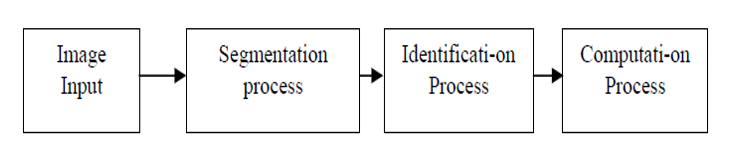
\includegraphics [scale=0.8] {flow_chart.PNG}
\caption{Diagram of image processing procedures}
\end{figure}



The paper didn’t say much about the procedure that is used to obtain the results but it explains the steps that they followed to get the results. According to their methodology they followed the following steps that are mentioned below.

\begin{enumerate}
	\item	Obtained or captured a digital image.
	\item	Performed image processing operations on image data.
	\item	Analyze and interpreted the image and use the results to get the body length, chest circumference and then use the standard formula to calculate the weight of cattle. 
	
\end{enumerate}

	The overall structure of the image processing method to get the weight of beef cattle can be demonstrated by the following block diagram [3]. \\
	


\begin{figure}[h]
\centering
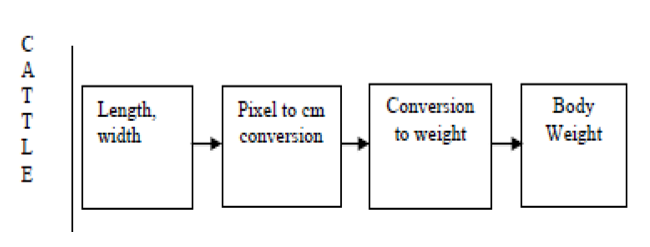
\includegraphics [scale=0.8] {blk_diagram.PNG}
\caption{Diagram of general process to Weighting the Cattle}
\end{figure}
	
	
	This paper cites some other research papers and explains the relationship between the body length and chest circumference. It gives reference to some formulas that can be used to determine the body weight of cattle. The author cites this research paper and according to Soeprapto [2], the body weight of cattle can be calculated by the formula:
	
	\begin{equation}\label{key}
		BW = \frac{BL + (CC)^{2}}{10840}
	\end{equation}
\textit{Where,}
\textit{BW} is the \textit{body weight} in kg \\ 
\textit{BL} is the \textit{body length} in cm \\ 
\textit{CC} is \textit{chest circumference} in cm \\

It cites another paper and says that according Schoorl written by Siregar [1], weight can be obtained by getting the physical dimensions of cattle. 
	
\begin{equation}\label{key}
BW  = \frac{(WoC + 22)^{2}}{100}
\end{equation}
Where, \textit{BW} is the \textit{body weight} in kg
\textit{WoC} is the \textit{width of chest} in cm


The author used the standardized formula based on the variables namely body length and chest width of cattle and obtained the results. He, in his paper claims that the results that were obtained by using this approach were not significantly different from the results of weighing using mechanical instrument [3]. 
\begin{center}
\textbf{	Weight Estimation Using Image Analysis and Statistical Modelling: A Preliminary Study}
\end{center}

The research was conducted previously on this topic and showed that there exists a correlation between the weight of the pig and physical features such as pig’s length or two dimensional area when viewed from above. This paper tries to find the correlation between the body weight of cattle and its physical features.\\

In the paper [4], the author automated the weight estimation system by using image processing techniques. The steps that are used in this approach as a part of image processing are following.

\begin{enumerate}
	\item 	Object Detection
	\item	Segmentation
	\item 	Filtering 
	\item	Feature Extraction 
	
\end{enumerate}


\textbf{Object Detection} \\

For the object detection, the author mentioned the calibration process that they used in their project. For calibration they set a fixed threshold. This threshold was determined by an offline calibration step. To complete this step, they took two images from a fixed camera rig; one image containing pig and other without pig (just of the background). These two images were used to locate the largest region of significant difference. Then they compared both images and based on the comparison results, a binary image was formed. Then a threshold was set based on brightness values in the binary image.  They author suggests a method to detect the pig in his paper. According to this paper [4], Pig detection could then be performed by sampling an image and comparing the measured brightness from the pixels in the defined detection region with the detection threshold. If a large percentage of pixels passed the test, then a pig was declared to be present and the image saved for further analysis. 

\begin{figure}[h]
\centering
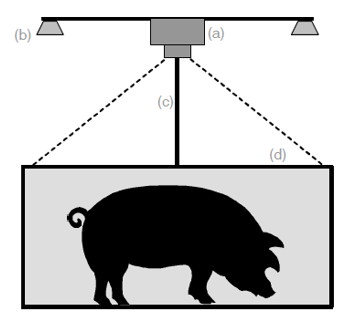
\includegraphics [scale=0.8] {camera_cali.PNG}
\caption{Camera and lighting setup}
\end{figure}


	
\textbf{Segmentation}

In the paper, fixed threshold method was used for segmentation. The author says that since the method was not entirely effective so in order to get the better results post filtering method was used to separate the object from the rest of the image. 
	
\textbf{Filtering}
	
Once the image is segmented, the post processing is required to clean up the segmented image. The post-processing involves two forms of filtering; median filtering and morphological filtering. A median filter is able to correct isolated segmentation errors, thereby “filling in” missed detections without causing great distortion to the image. It was also used to prevent the next process, image opening, from having a detrimental effect. After applying median filter image opening process was applied. 


\begin{figure}[h]
\centering
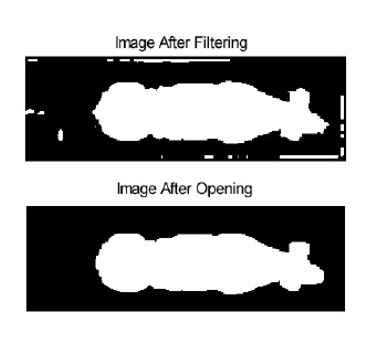
\includegraphics [scale=0.8] {image_open.PNG}
\caption{Image filtering and opening performed on the image of pig}
\end{figure}


	
\textbf{Feature Extraction}


After doing segmentation, the features were extracted to estimate the weight of cattle. The features that were employed in this study were area, length and spine length. The area of the object in pixels is trivially defined to be the sum of the binary pixel values over the whole image. This assumes that by this stage there will be only one contiguous region in the image.
The spine length was computed by isolating the largest branch in the skeleton and counting the number of pixels. The main branch was located by determining the location of junctions via a zero-crossing method [5]. 



\begin{figure}[h]
\centering
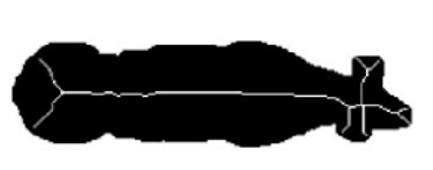
\includegraphics [scale=0.8] {skeleton.PNG}
\caption{Skeletonization performed on a segmented image}
\end{figure}


The length feature refers to the distance from the center of the pig’s neck to its tail. The position of the pig’s neck proved to be difficult to detect due to the unknown orientation of the pig’s head. It was decided to estimate the pig’s neck position as the point at which the main segment (referred to as the spine above) of the pig’s skeleton terminated. After skeletonization as above, the two endpoints of the spine were found [4]. \\
The “head” endpoint was deemed to be the one which gave rise to the most sub-branches, as the head was more topologically complex than the rump and usually produced a more structured sub-skeleton. The tail was assumed to be the most extreme pixel of the segmented image at the opposite end from the head. With these two data points the Euclidean distance could then be found, giving a close approximation of the length of the pig. Euclidean distance was appropriate since the pixel dimension ratio was one-to one [4]. \\
According to the author, the best results were obtained when using the neck-to-tail distance versus log weight (correlation coefficient 0.5640) and area versus weight (correlation coefficient 0.5295) to determine the weight. These correlation coefficients were both significant, having a probability of occurrence less than 1\%. The resulting linear weight prediction formulas achieve an average absolute error just under 5\% [4]. The author says, it confirms the claim that there exists a correlation between physical features and body weight. 

\begin{center}
	\textbf{Beef Cattle Weight Determine By Using Digital Image Processing} 
\end{center}


The body length, chest circumstance, height and width of the animal could be estimated.


\textbf{Image Preprocessing:}
The paper first did some image preprocessing depending on the image of cattle to make it segmented to do further calculation. 
Once the image is segmented it is divided into segmentation parts as shown in the figure below. [6]

\textbf{Suggested Segmentation Division:}

\begin{enumerate}
	\item Round and rear shank
	\item Sirloin, short loin, tenderloin, top sirloin, bottom sirloin, flank
	\item Rib and short plate
	\item Chunk, brisket and front shank
	


\begin{figure}[h]
\centering
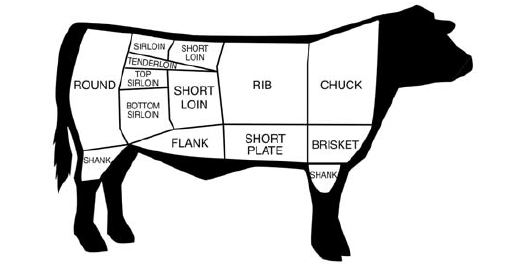
\includegraphics [scale=0.6] {beef.PNG}
\caption{Types of Beef}
\end{figure}
	
\end{enumerate}

\textbf{Methodology:}


\begin{enumerate}
	\item Localized Region Based Active Contour
	
	Segmentation method that minimizes curves in the segmentation process.
	
	\begin{equation}\label{key}
	E_{snake}= E_{internal} + E_{external} + E_{constraint}
	\end{equation}
	
	Make an initial contour surrounding the object, then with the energy of an object image (External) will cause the curve shrink and follow the pattern of the object. The curve can be moved closer towards the object and adjust the shape of the object because of the energy on the curve (Internal). Use active contour without edges which does not depend on the value of the gradient image as a condition to stop the contour changes. This model uses the average energy in the region. [6]
	

\begin{figure}[h]
\centering
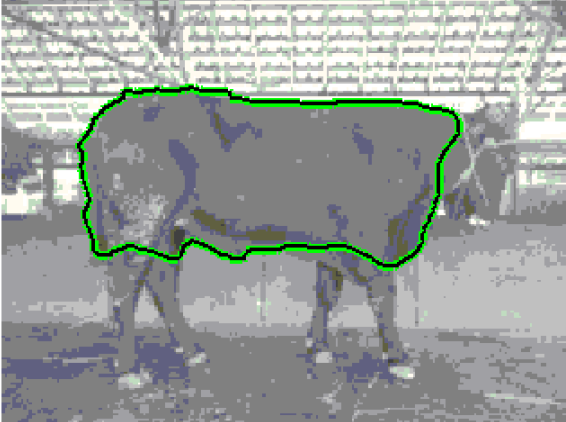
\includegraphics [scale=0.6] {contour.PNG}
\caption{Objects covered by the curve cantour}
\end{figure}
	
	\item Linear Regression
	
	Fitting a linear equation to observed data on two variables: explanatory variable, and dependent variable. Use scatter plot to determine whether or not there is a relationship between the variables of interest.[6]
	
	\item  Calculation Process
	
	To calculate the weight of each part, the part of side picture of cattle feature will be regressed with chest feature data.[6]
	
	The results that were obtained from this approach were as follow. 
	\begin{enumerate}
		\item	73.213\% accurate system;
		\item	Accuracy between segmented object and without segmentation is the same because of anatomical shape. 
	\end{enumerate}
	
	
\end{enumerate}

\begin{center}
		\textbf{Estimation of Calf Weight from Fixed Point Stereo Camera Images using 3D Successive Cylindrical Model}
\end{center}


In order to improve productivity, the objective is to simplify the estimation of calf weight. In this paper, method to estimate weight by three-dimensional model of cattle shape using stereo images is proposed. This enables to solve the problem that requires no special environment to shoot images only from above in the previous work. Moreover, it can mitigate the issue of the posture of cattle by grasping it three-dimensionally. In the proposed method, firstly, the stereo camera is created by fixing two network cameras. The image of the calf is taken by these cameras, and the stereo matching method is applied to the captured image to calculate three dimensional coordinates. Next, only the body is modelled because chest girth and waist girth have the highest correlation with weight. Since the body has a rounded shape, a three-dimensional successive cylindrical model is used. Weight estimation by using the linear regression equation between the volume of the obtained three-dimensional successive cylindrical model is obtained and the weight measured manually. [7]

\textbf{Basic Information of Cattle Body and Extraction of Body Parts Data}


Two fixed network cameras shoot motion images of calves. These motion images are divided into frames and analysed as static images. The image can be used as a stereo image by calibration of cameras. In stereo matching, the distance between the camera and the target object is kept constant. This distance depends on the size of the target object. In this paper, the distance ranged from 1 to 3 meters. [7]




\begin{figure}[h]
\centering
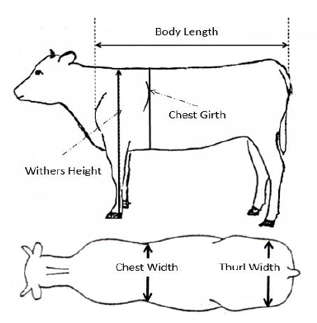
\includegraphics [scale=0.8] {parts}
\caption{Each parts of cattle body}
\end{figure}


Two methods are used to extract body parts of the cattle from the stereo images. First method is background subtraction method where the background image is taken in advance. Second method is using parallax values obtained from the stereo matching method.
Both of these methods output mask images. The common part of these two mask images is taken to extract the cattle body. This process eliminates the noise. The output image is converted to binary to give cattle body in white and remaining in black. 




\begin{figure}[h]
\centering
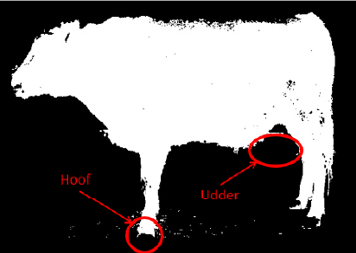
\includegraphics [scale=0.8] {bin_img.PNG}
\caption{Binary image of cattle}
\end{figure}


\textbf{Modeling Body of Cattle}

Measuring chest girth precisely is difficult so it model the entire body using a successive cylindrical model to find correlation with weight. Three-dimensional point cloud data is calculated from stereo images using the stereo matching method. Surface of cattle is smooth with little change in colour, therefore the errors are high and volume cannot be determined precisely. Therefore, we attempt to model it by using a simple and fixed three-dimensional model. [7] A cylindrical model is chosen since it best models the rounded shape of the cattle body. It is necessary to divide the body into several parts in order to change the radius of the cylindrical model according to the position in the x direction of the body. [7]




\begin{figure}[h]
\centering
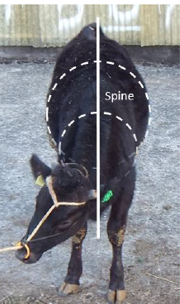
\includegraphics [scale=0.8] {front.PNG}
\caption{Cattle from above}
\end{figure}


The radius of the cylindrical model is determined by using the circle closest to the point cloud data. This enables to detect the body shape while reducing errors. To develop the circle nearest to the point cloud data, a circle fitting using a generalized Hough transform is employed. 




\begin{figure}[h]
\centering
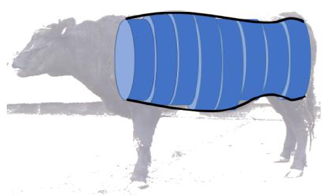
\includegraphics [scale=0.8] {spiral.PNG}
\caption{Successive cylindrical model}
\end{figure}


First, when comparing the cases where the body is divided and not divided, the correlation coefficient and the average error are better when divided. Then, comparing the case where each result was individually examined and the volume was averaged, all of the result was better when the volume was averaged. Thus, it verified the effectiveness of slicing the image of the body with the proposed method and to shoot and use multiple images of the same cattle. [7]
The experimental results have revealed the following: 

\begin{enumerate}
	\item There is a correlation between weight and volume obtained by modeling the body. 
	\item The proposed method that models by slicing the image of the body is highly effective. 
	\item There is a possibility to improve accuracy of weight estimation by using multiple stereo images
	
\end{enumerate}

\begin{center}
	\textbf{	Weight Estimation through Image Analysis}
\end{center}

In this paper [9], image segmentation based technique has been used to segment out the region from the image and then using the dimension of the image object weight has been calculated using density based formula. According to the author, it was observed through this experimental process, results were 92\%-94\% accurate. [9] \\
The strategy that is used in the paper can be understood by the following flow chart diagram.



\begin{figure}[h]
\centering
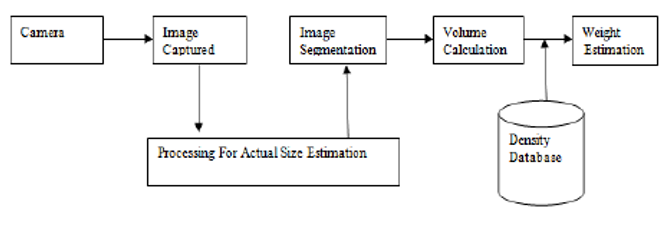
\includegraphics [scale=1.0] {flowChart.PNG}
\caption{Process Flow Chart}
\end{figure}



The propose strategy in paper [9] consists of the following steps. 

\begin{enumerate}
	\item 	Pre-Processing
	\item 	Image Segmentation
	\item 	Volume Calculation 
	\item 	Mass Calculation
\end{enumerate}

\textbf{Pre-Processing}\\
The image is a 2D array which consists of finite and discrete pixel values. In order to segment out the foreground object (cattle in this case) from background some pre-processing is required. In pre-processing phase the image is downscaled for faster computation. The pre-processed image is segment using K-means clustering algorithm to extract the object from the image. The image is divided in which subtraction of the image comprising the object cluster is used for further processing. [9]


\textbf{Image Segmentation}

In this phase, the image that was obtained from the pre-processing step is then segmented using watershed segmentation algorithm to extract the object from the image.  

The paper [9] explains the method that is used to calculate the volume in detail. Let f(x, y) be the input from the front view and s(x, y) be the input from the side view which is then preprocessed to get f`(x, y) and s`(x, y). These preprocessed images are passed through the segmentation function, as mentioned above, to get clustered images of front and side view, that is g(x, y) and h(x, y) respectively. The subsection of g(x, y) and h(x, y) containing the object’s cluster. The grid area technique is applied on the segmented images. The M x N subsection is selected for grid area calculation. The subsection consists of object’s cluster O and background cluster G is further divided into smaller grid of size m x n. The M x N is then iterated for every grid and for each grid if more than 50\% pixels in the grid belong to object’s cluster O then the grid is considered to be a part of the object’s cluster. The iteration gives the total number of grids belonging to O, that is, O[n]. The count O[n] is stored in a vector for every column in the grid array. The grid area returns two vectors, $C_{ocside}$ for side image and $C_{ocfront}$ for front image. After applying this technique, the following cases might arises. 


\begin{enumerate}
	\item The vector have equal dimensions 
	\item The vector have unequal dimensions
	
\end{enumerate}

\textbf{Volume Calculation}

If the dimension are not equal then extra elements from the larger vector are removed and average of these elements is inserted back into vector. 
Volume can be calculated using the following formula. 

\begin{equation}\label{key}
Volume = (\sum_{i=0}^{n} C_{ocfront} (i) + C_{ocside}(i)) * V_{grid} * sf^{3}
\end{equation}
$ Where,  V_{grid} =$ \textit{Volume of the grid cube}\\
$sf = \textit{Scaling Factor} $
\\

\textbf{Mass Calculation}

Using the volume of object obtained from the above mentioned process, the mass can be calculated as follow.

\begin{equation}\label{key}
Mass = Density * Volume
\end{equation}

\pagebreak 

\begin{center}
\textbf{Learning Deep Features for Discriminative Localization}
\end{center}


\paragraph{}In this research paper, we visit the global average pooling layer and shed light on how it explicitly enables the convolutional neural network (CNN) to have 
remarkable localization ability despite being trained on imagelevel labels. While this technique was previously proposed as a means for regularizing training, 
we see that it actually builds a generic localizable deep representation that exposes the implicit attention of CNNs on an image. Despite the apparent simplicity of global average pooling, we are able to achieve 37.1\% top-5 error for object localization on ILSVRC 2014 without training on any bounding box annotation. We can see in a variety of experiments (given below) that the network is able to localize the discriminative image regions despite just being trained for solving classification. [8]

\begin{figure}[h]
\centering
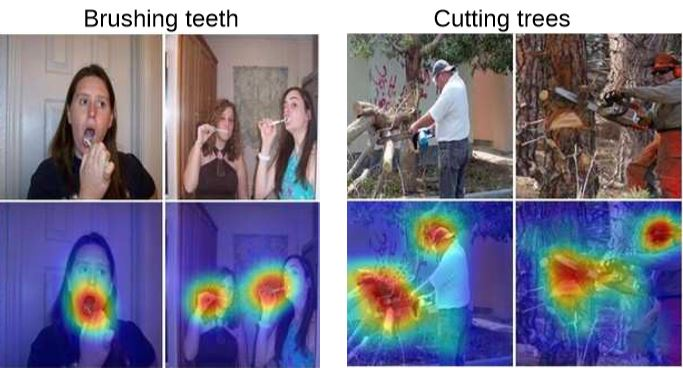
\includegraphics [scale=0.8] {Figure1.jpg}
\caption{Simple modification of the global average pooling layer combined with our class activation mapping}
\end{figure}

\paragraph{}The final output above is called Class-Activation-Map(CAM). It is actually the regions of the image that are the deciding factors during classification i.e. 
Discriminative-Regions (DR). These maps are calculated by first finding the node with the highest classification score and then finding the weights that connect 
the neurons from Global Average Pooling (GAP) layer to the final layer (classification layer). We can then find the linear combination of these weights and feature maps obtained from the last convolutional layer to find the CAM. The figure below illustrates that.

\begin{figure}[h]
\centering
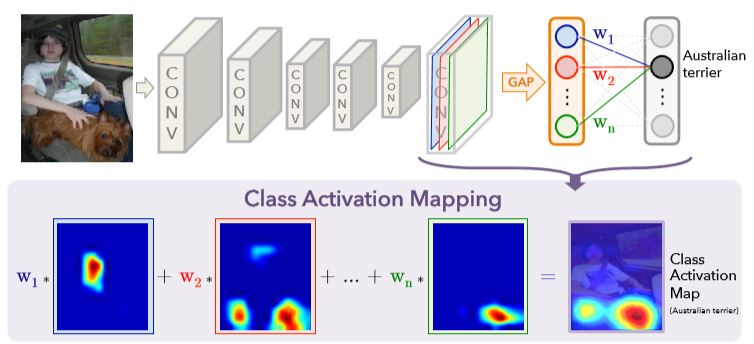
\includegraphics [scale=0.8] {Figure2.jpg}
\caption{Class Activation Mapping: the predicted class score is mapped back to the previous convolutional layer to generate the classactivation maps (CAMs). The CAM highlights the class-specific discriminative regions}
\end{figure}

The results shown are evident that localization problems(with reliable results) can be solved by using a vanilla CNN without going into the complexity of object detection.[8]



\section{Conclusion}

The research papers we reviewed did not incorporate the depth information which in our case would greatly increase accuracy. To counter this, we explored 3 different approaches in order to predict the weight of the cattle as accurately as possible.

\subsection{Approaches}

\subsubsection{Automated Heart Girth Measurement Where depth is Fixed}

The heart girth measurement is the most reliable technique of estimating the weight. In this approach, we take two variables; Heart Girth and the Body Diagonal. We assume that the depth of the animal i.e the distance of the animal from the camera is either known or fixed. We take two images, the front view and the side view. The width of the animal is determined from the front view. To get both the variables, we convert the number of pixels in the image to real-world measurements using the formula described in curve length estimation section. 

The following vectors are obtained from the images:

\begin{center}
$\vec H = [p1, p2, p3 ... pN]$\\
$\vec D = [dp1, dp2, dp3 ... dpN]$
\end{center}
Where H = Heart Girth Pixel Vector and D = Diagonal Pixel Vector.

\subsubsection{Heart Girth Measurement with Per-Pixel Depth}

This approach builds upon the previous approach. We take the same variables i.e the Heart Girth and the Body Diagonal. This method however requires only 1 image; the side view of the animal. We find the inner and outer bounding boxes around the required parts of the animal. The curvature of the animal is estimated using the per pixel depth information. 

The following vectors are obtained from the images:

\begin{center}
$\vec Hp = [p1, p2, p3 ... pN]$\\
$\vec Dp = [dp1, dp2, dp3 ... dpN]$

\end{center}

Where H = Heart Girth Depth per Pixel Vector and D = Diagonal Depth per Pixel Vector.



\subsubsection{Curve Length Estimation:}

In the above mentioned approaches the final result we get is a bounding box from our core component using our deep learning model which encapsulates the information of body length in the diagonal and heart girth measurements in height of the box. Since these values are just only represented by two pixel coordinates top-left and bottom right. As mentioned earlier to get the measurements accurate we have to incorporate the depth information. Since we have depth map and RGB image of same dimensions and from same camera we can safely map this bounding box to depth image as well. 

Once we have a this image box on depth image we will extract out the vector of pixels from the heart girth line of the bounding box and diagonal vector from pixels starting from bottom left and the top right  point in this image.
Once we have these two vectors we can convert it into real world measurements using the procedure defined below in Appendix.B, Math section. 

 






\chapter{Software Requirement Specification (SRS)}
\label{chap:srs}
\section{Introduction}
\subsection{Purpose}

The purpose of this document is to present a detailed description of our Final Year Project, InstaWeight. It will explain the purpose and features of the system, the core components and the interface of the system. It will give in-depth information of our system that we will developed. 

\subsection{Scope}
The aim of the system is to estimate the weight of the cattle accurately. The system is designed to automate the process of measuring cattle’s weight on a large scale in a farm. Moreover, it will keep track of the daily growth of the cattle’s weight to take decisions related to live stock business. The core component of the system will be responsible to detect the features of the animal from the image to estimate/predict the weight of the animal. This core component will be developed using machine learning and image processing algorithms. 

\vspace*{2mm} On client side, there will be a admin panel to the store the weight of cattle and see the growth trend of each cattle. The system will also contain a relational database containing the basic information such as id, age, gender, weight etc. of each cattle. 

\subsection{Overview of the document}
The next section of this document, ‘the overall description’ gives an overview of the functionality of the system. It describes the functional and non-functional requirements, use case diagrams, system diagram and external interfaces. 

\section{Overall Description}

\subsection{System Environment}

The autonomous weight estimating system has two active actors a system with three components. A normal user/ farmer can capture the image of a cattle to measure the weight of an animal. The camera would be connected to the core component of the system. The weight would be saved in admin panel. The owner of the farm or a rancher can access the admin panel to keep track of the growth of the cattle.\\



\begin{figure}[h]
\centering
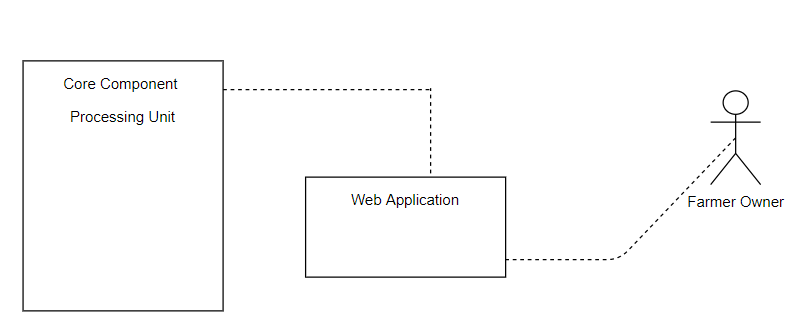
\includegraphics [scale=0.6] {ed.png}
\caption{System Environment Diagram}
\end{figure}


\pagebreak

\section{Functional Requirements}

\subsection{Business Requirements}

\begin{enumerate}
\item The system should be 90\% to 95\% accurate.
\end{enumerate}

\subsection{Web Application (Admin Panel):}

	The core functionalities of admin panel would be following: 
\begin{enumerate}
	\item \textbf{Authentication:}
	\begin{enumerate}
		\item The sign up of all users would be done by the admin panel. 
		\begin{enumerate}
			\item To sign up into the system, the basic information of the user would be required and will be added to the system. 
		\end{enumerate}
	\end{enumerate}

	\item \textbf{Dashboard:}
\begin{enumerate}
	\item The admin panel would display the overall growth of all cattle in last six months through pi-chart. 
	\item It would show the growth progress of each cattle on individual level in last six months. 
	\item Admin panel would have different tabs and button to add, update and delete.
	  \item Record of the animal can be update by clicking on the “Update Record” tab. 
	 \item The cattle’s record can be deleted by “Delete” button. 
\end{enumerate}

	\item \textbf{Cattle Management: }
	
	\begin{enumerate}
		\item \textbf{Add Cattle}
		\begin{enumerate}
			\item To add an animal into the system, it would be required to add some details such as age, gender, type etc. into the system.
		\end{enumerate}
		\item \textbf{List View}
		\begin{enumerate}
			\item List of all animals would be displayed.
		\end{enumerate}
		\item \textbf{View Details}
		\begin{enumerate}
			\item On clicking view details, the complete details of every individual animal would be displayed on screen. 
		\end{enumerate}
\end{enumerate}
	
	\item \textbf{Under Observation:}
	\begin{enumerate}
		\item All cattle who are diagnosed ill or under stress by the system and needs checkup. 
	\end{enumerate}
	
	\item \textbf{Settings:}
	\begin{enumerate}
		\item Personal configuration section from where admin can change password and other login details. 
	\end{enumerate}
	
\end{enumerate}



% --- The above is to be modified as per your project, e.g. a flat list if your system has limited functional requirements.

\section{Non-functional Requirements}

\hspace*{10mm} Following are the non-functional requirements of our system. 
\begin{enumerate}
	\item \textbf{Security:}\\
	The user's data that would be required during sign up should be confidential, safe and secure.
	\item \textbf{Performance:}\\
	The system should less than a minutes to process the image and estimate weight.
	\item \textbf{Compatible:}\\
	The system should be compatible with all android devices. 
	\item \textbf{Memory Efficient:}\\
	The mobile application should be space efficient and should not occupy large space of memory.
	\item \textbf{Usability:}
	The interface of the system should be simple and flow of app should be understandable by farmer who is not well educated. 
	\item \textbf{Scalability:}\\
	The system should be scalable so that it can later be used in real world or at industry level. 
	\item \textbf{Maintainability:}
	The system should be easily maintainable so that it can become more advance and efficient when use in industry. 
	\item \textbf{Legal:}\\
	According to the intellectual property rights, the system should only be used by Folio3. 
	
\end{enumerate}

\pagebreak
\section{External Interfaces}

\subsection{User Interfaces}
\subsubsection{Admin Dashboard}

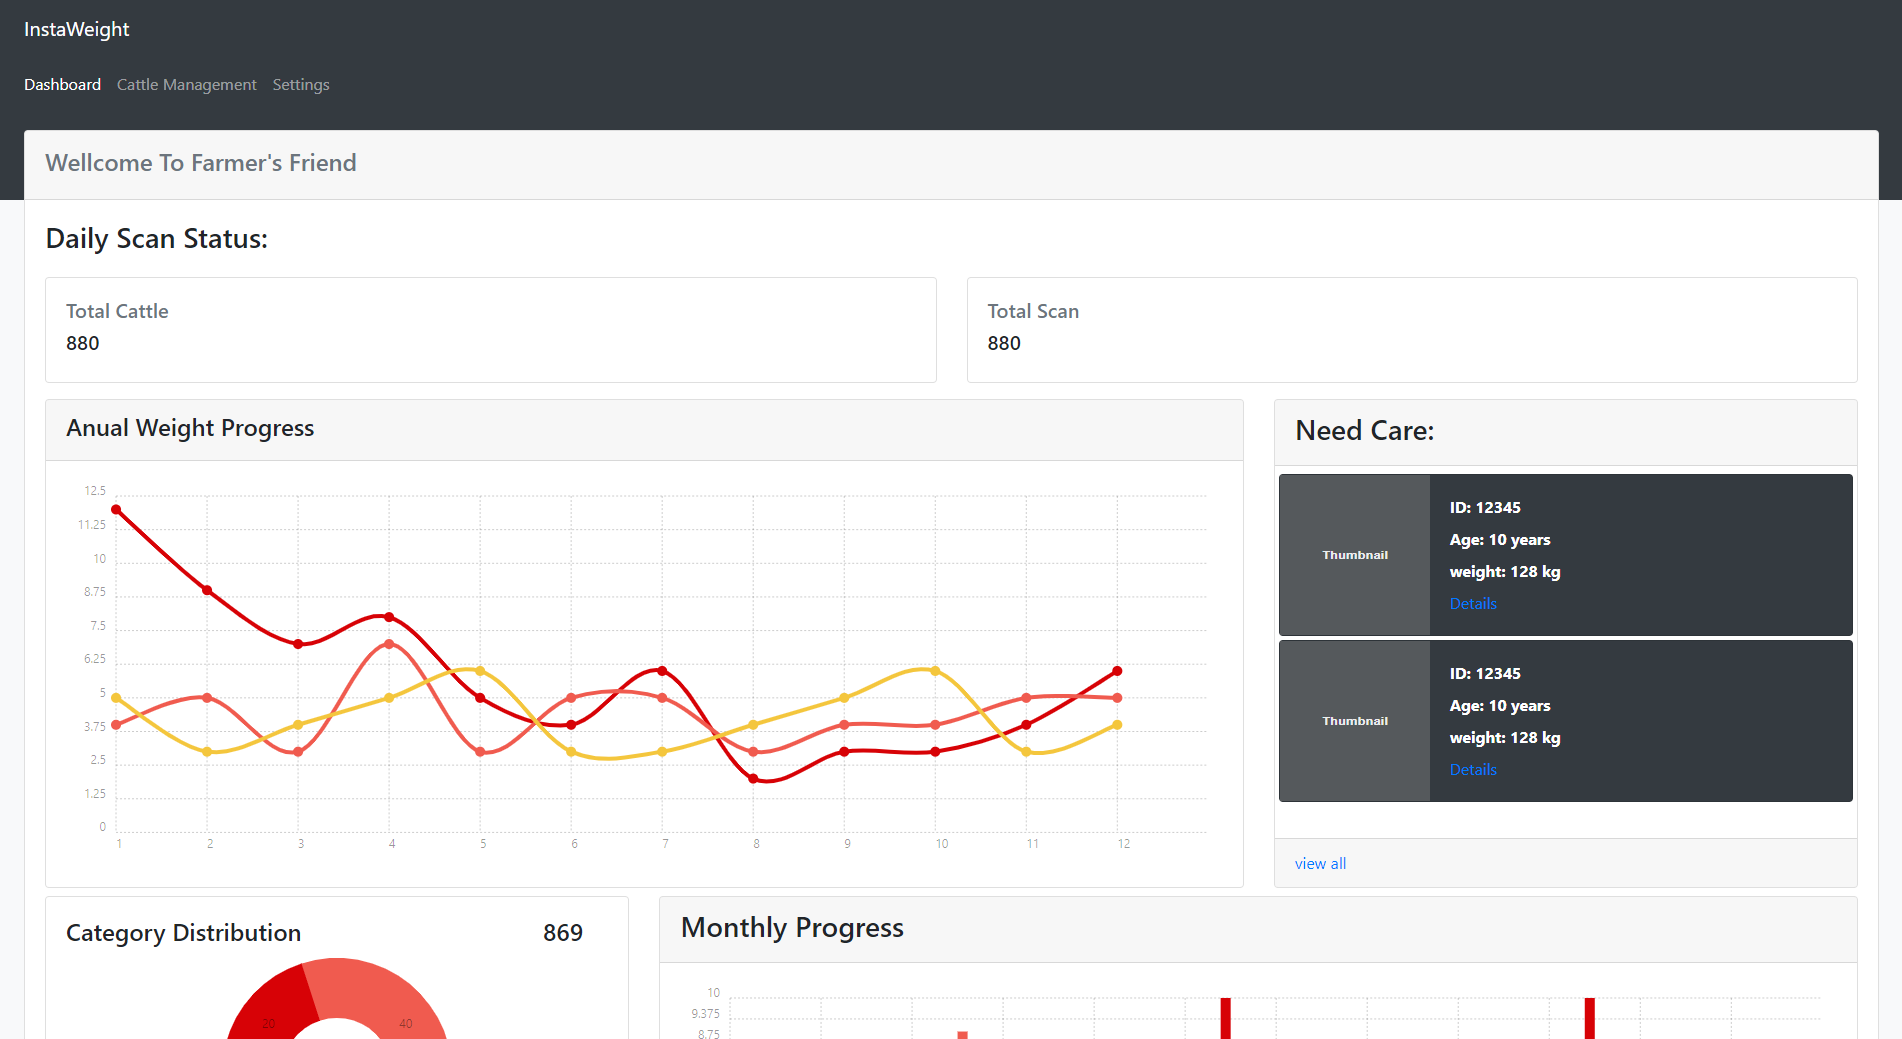
\includegraphics [scale=0.3] {dashboard-1half.png}

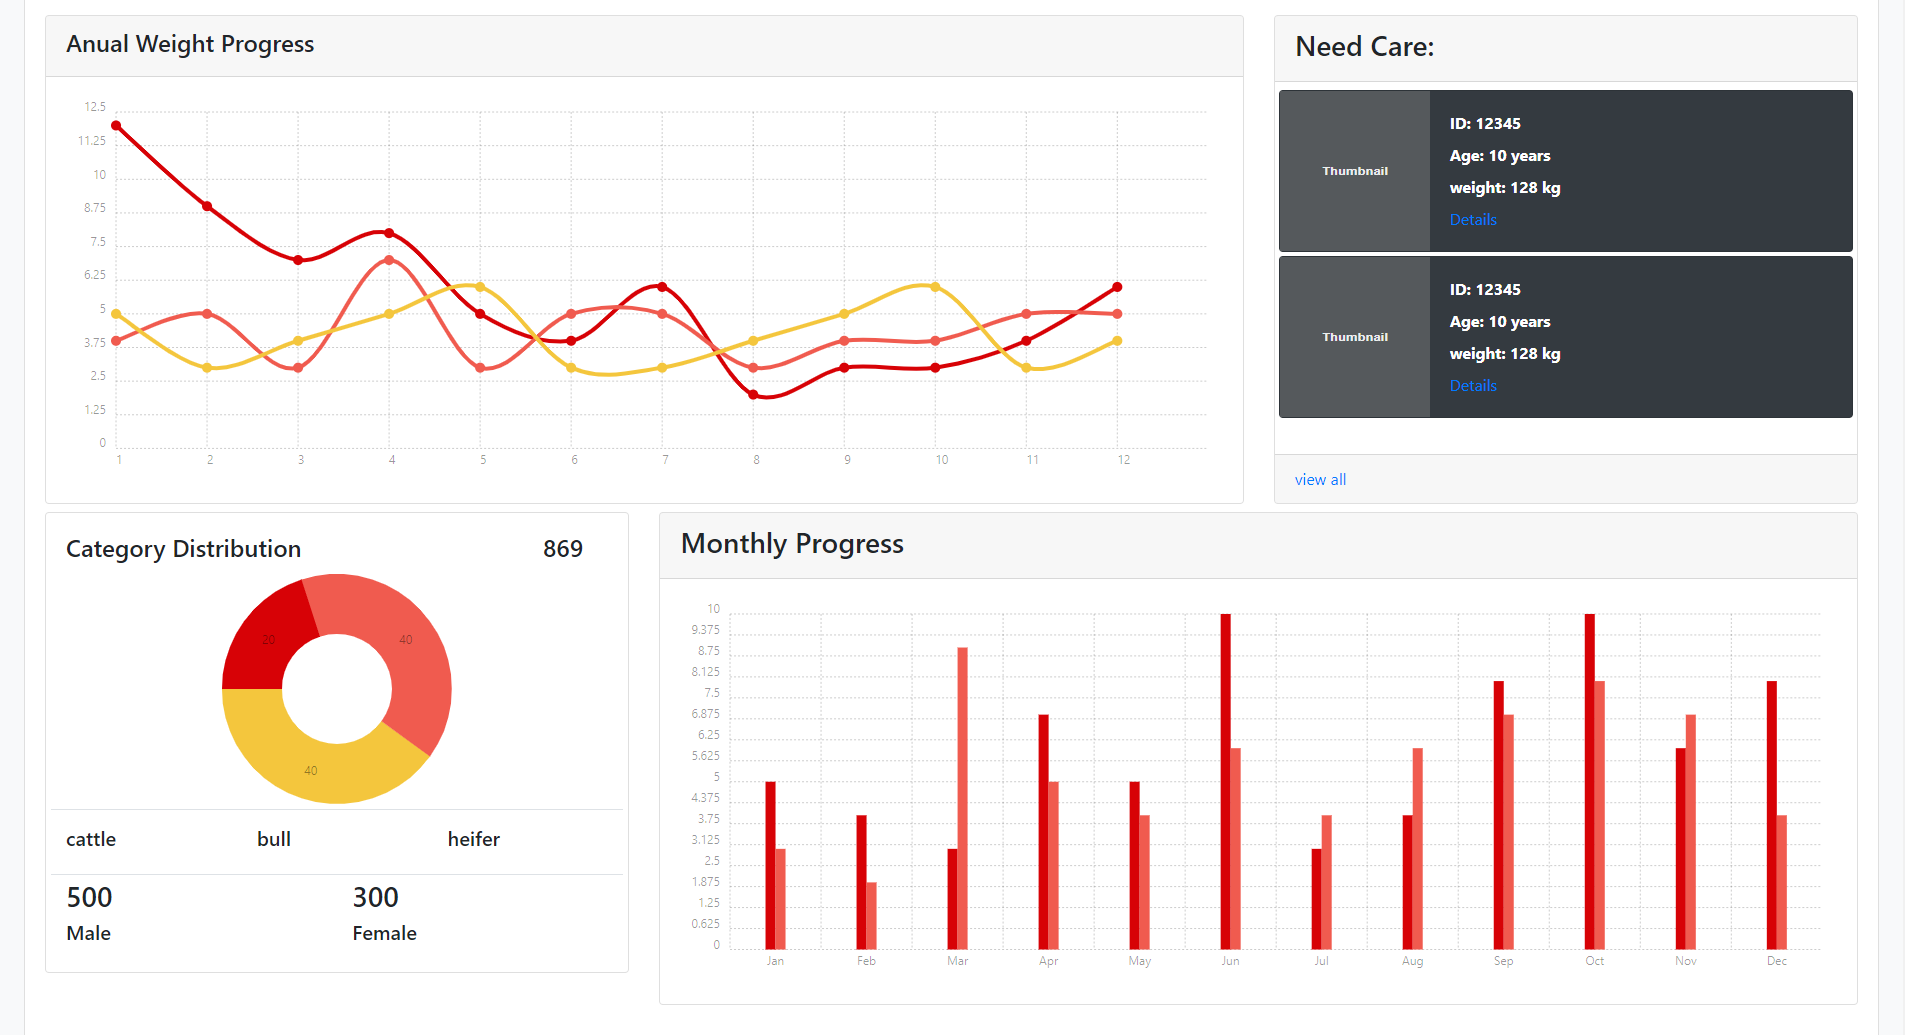
\includegraphics [scale=0.3] {dashboard-2half.png} \\

This page will display some graphes which will show annual and monthly animals' progress. it will also display animal which need special care. 

\newpage
\subsection{Cattle Management:}

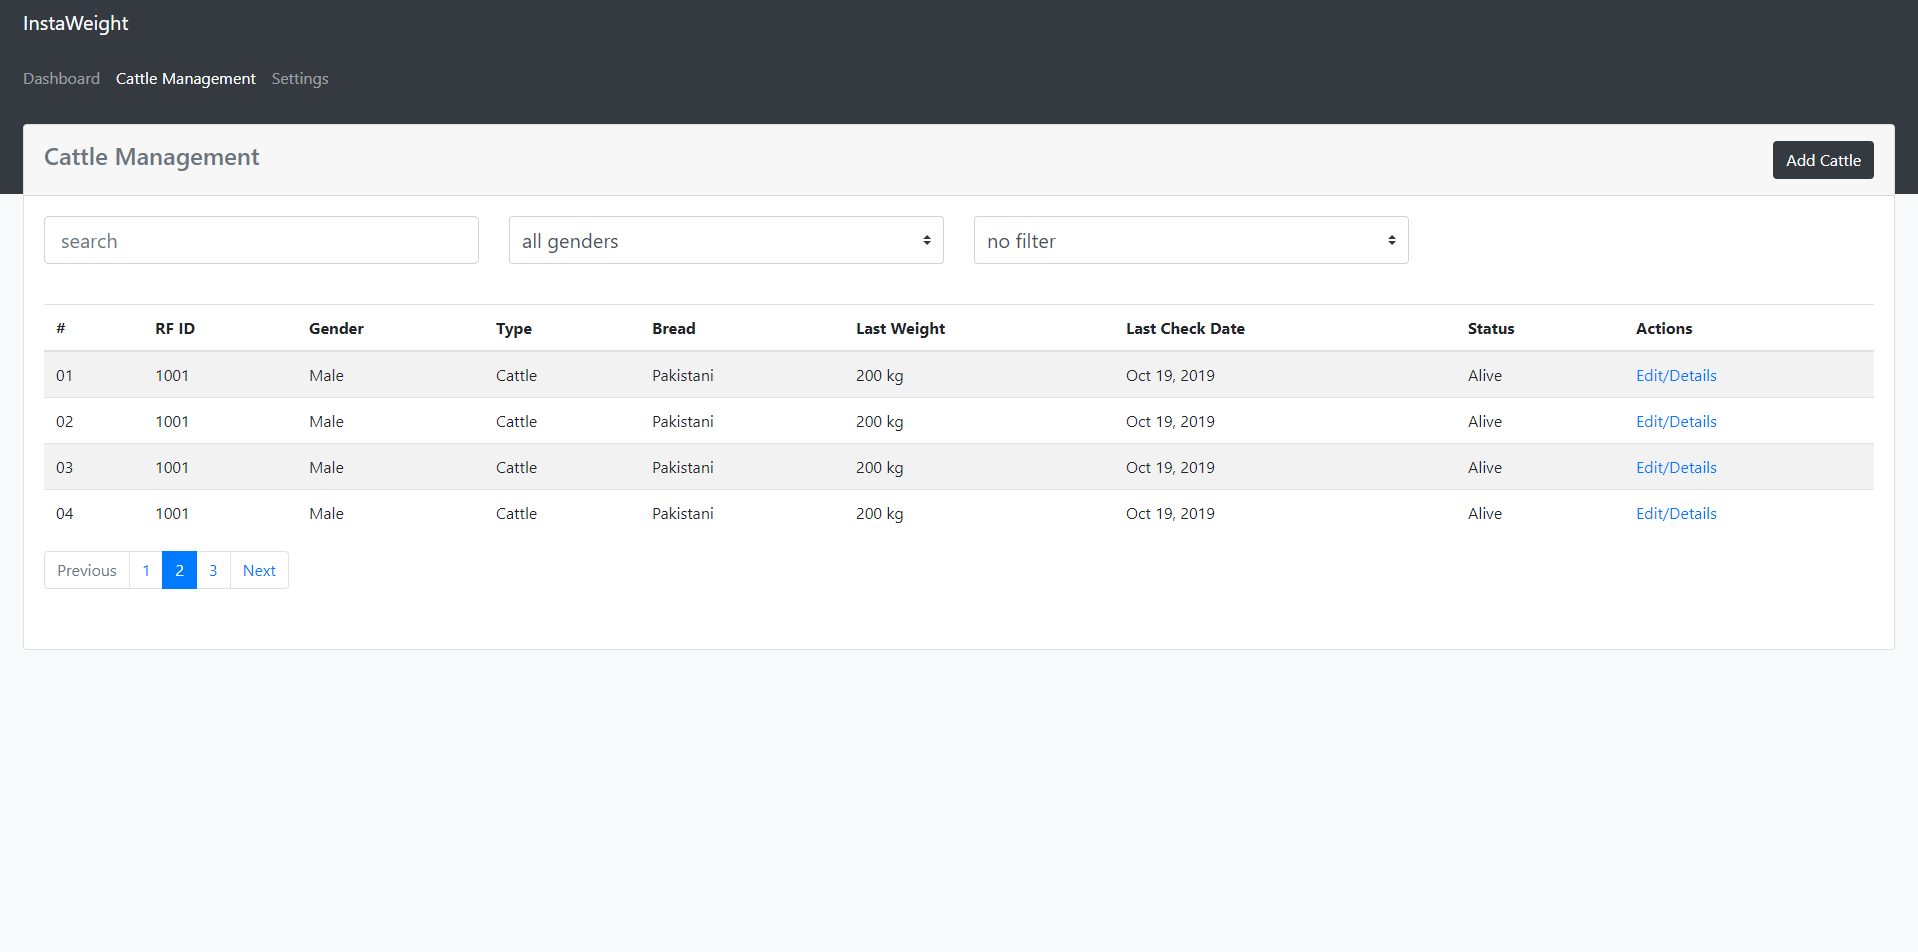
\includegraphics [scale=0.3] {cattle-management.png} \\

This will display all animals in a tabular form and will let user filter the animals and see their details.

\newpage

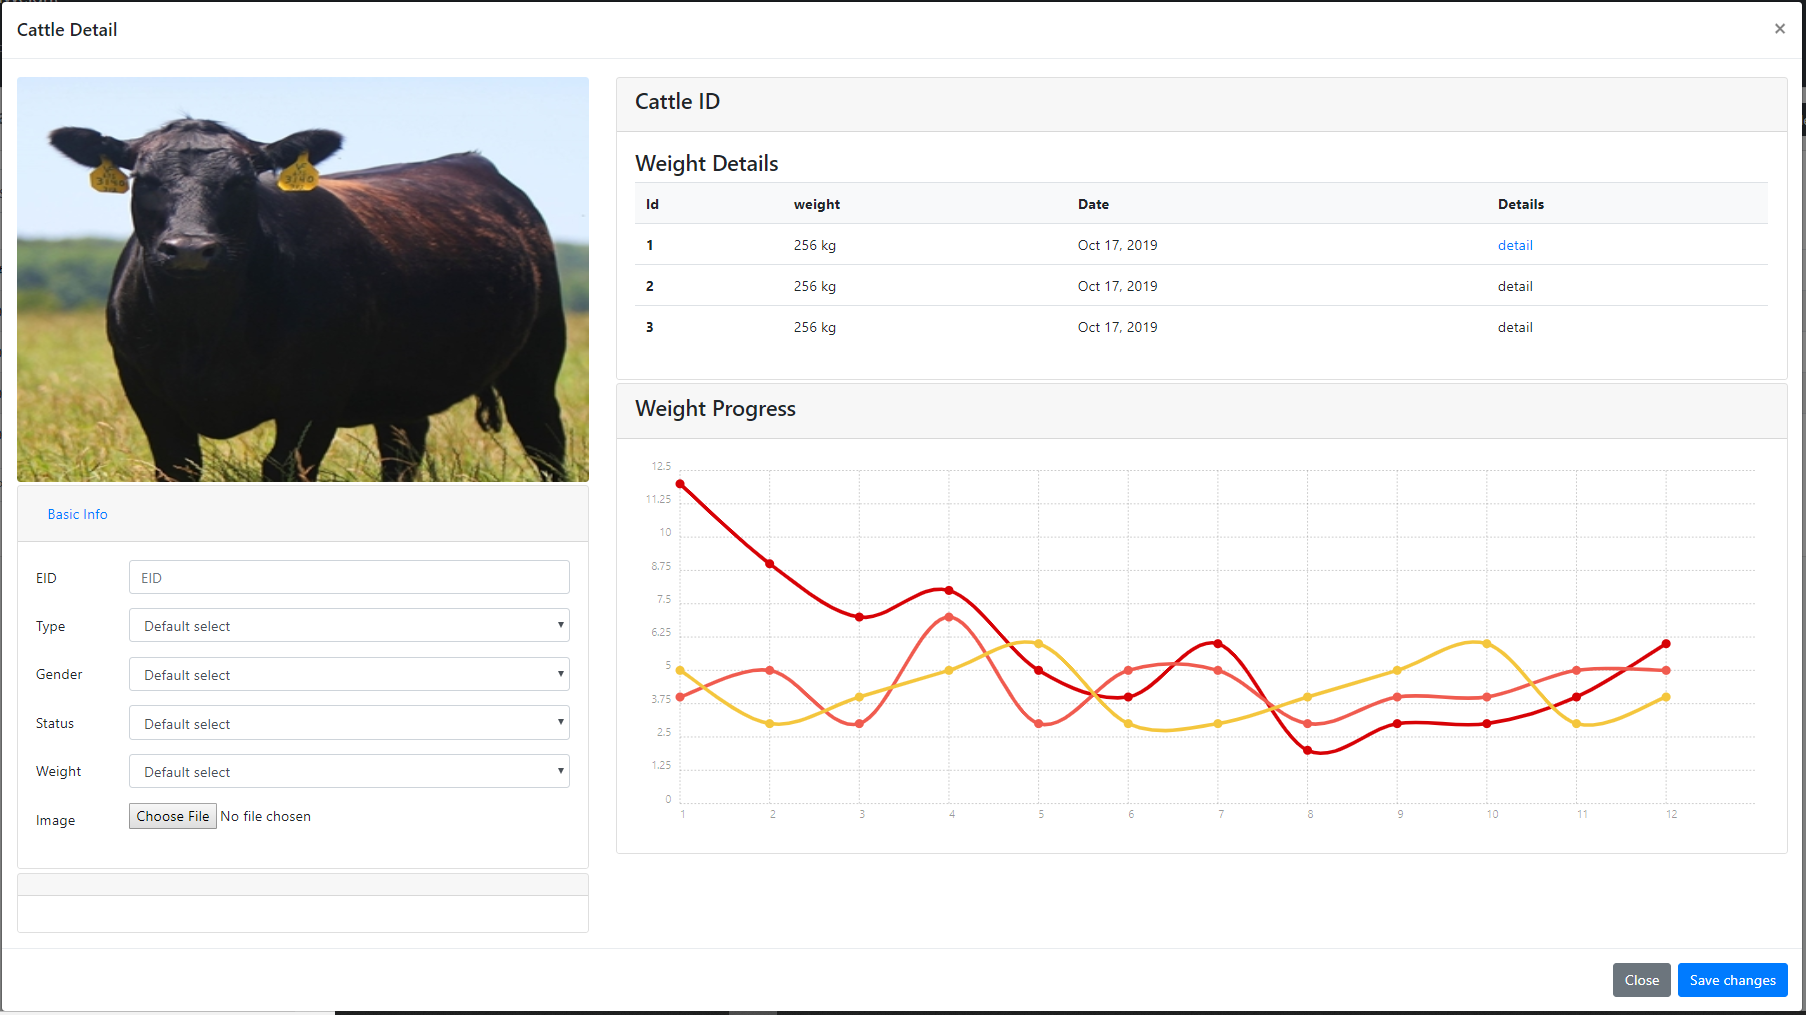
\includegraphics [scale=0.3] {details-modal.png} \\

This will display details of a single cattle and lets user edit it.

\newpage

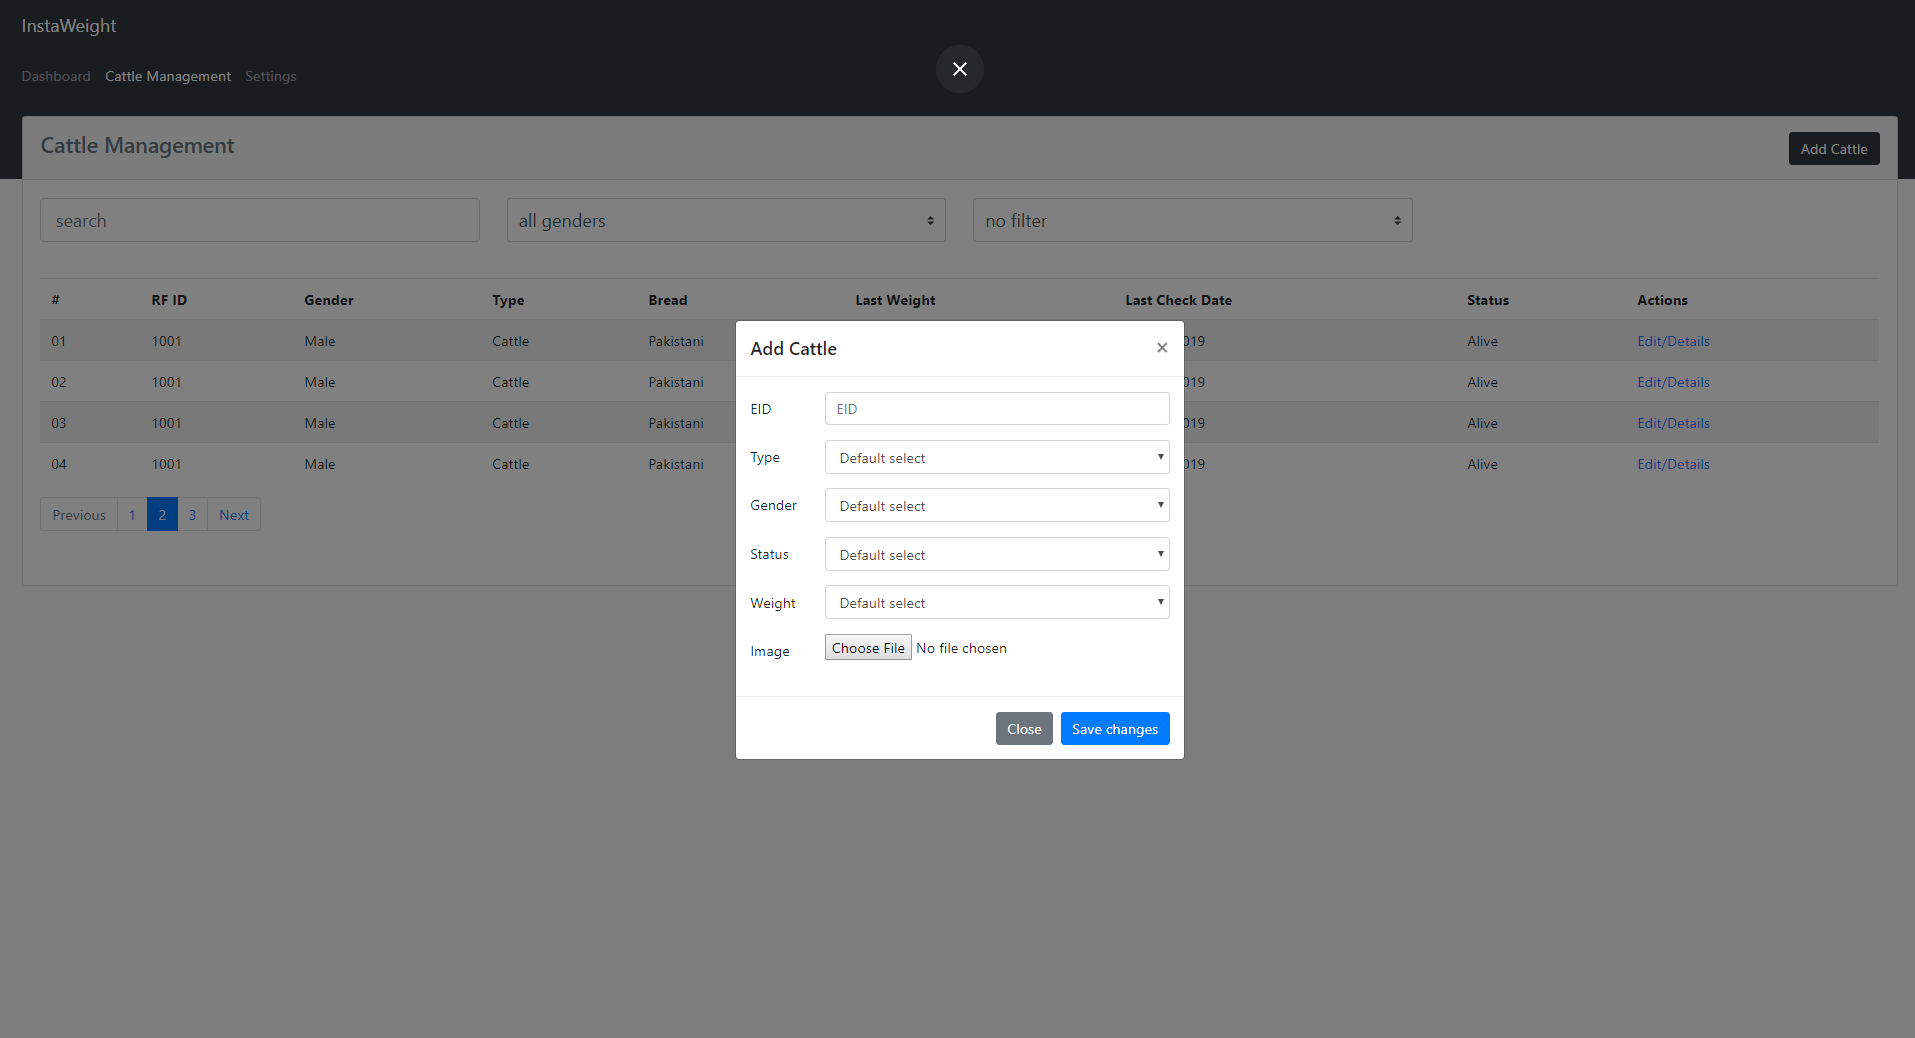
\includegraphics [scale=0.3] {add-cattle-modal.png} \\

This will will be the interface though which a new cattle can be added details of a single cattle and lets user edit it.

\newpage

\subsection{Dataset and Augmentation}
\subsubsection{Dataset Collection:}

The dataset was collected 3 times. Here are the details of the dataset:
\begin{enumerate}
\item \textbf{Dataset V1} - This dataset was collected on a farm having about 150 animals and approximately 1200 RGB images were collected. All of the dataset was annotated for two bounding boxes, one to enclose the whole cattle (outer bounding box) and the other to enclose abdomen of the cattle (inner bounding box). Out of those 1200 images 229 were usable. We also scrapped about 700 images from google and around 277 were usable. These images only consisted of a side view of the Cattle and no depth and weight labels were available. These images were used for inner and outer bounding box detection. We augmented this dataset by making each image brightened with gamma = 2.0. We then darkened the image and introduced noise to simulate low light conditions. The images were flipped on a vertical axes. hence generated 3 augmented images out of one. The total number of images after augmentation were about 2,024.
\begin{figure}[h]
\centering
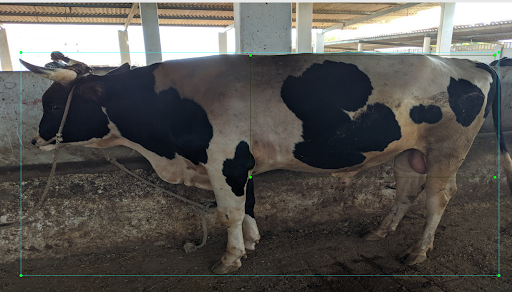
\includegraphics[scale=0.5]{datasetv1.jpg}
\caption{Annotation on V1 for inner and outer bounding box}
\end{figure}


\item \textbf{Dataset V2} - This dataset was collected on a farm having about 65 animals. Approximately 1235 RGB images with depth were taken. We annotated these images for the Inner and outer boxes as well as for Semantic Segmentation. These were also side views of the cattle and no informatio of cattle's weight was available. Total images in our dataset were 1235 with depth, 229 (original from V1 without depth) and 2,024 (including original, augmented and scraped images) without depth. These images were used for Semantic Segmentation and bounding boxes. 
\pagebreak 
\begin{figure}[h]
\centering
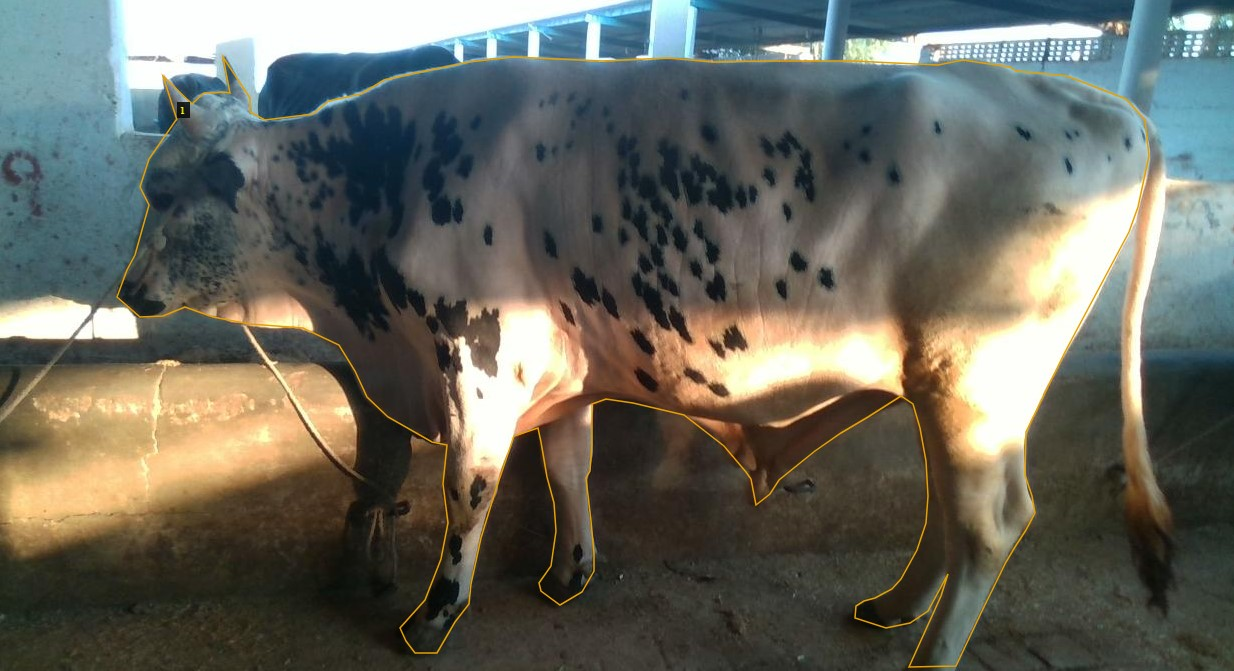
\includegraphics[scale=0.3]{maskRCNNAnnotation.jpg}
\caption{Annotation on V2 for mask RCNN}
\end{figure} 
\\

\item  \textbf{Dataset V3} - This dataset was taken urgently and only 8 animals were available. This dataset was created because the previous image with depth has some noise in depth values and a lot of zero values appear in the depth. The problem aroused because the camera was not calibrated correctly. After correct calibration, Approximately \textbf{1000} RGB images with Depth were taken. This dataset was also annotated for inner and outer rectangles but was only used for depth reated experiments. 


\end{enumerate}
\textbf{All of these images were annotated by our own team. We were unable to get cattle's weight labeled dataset because most of the farms do not keep it. And due to Covid-19 we were unable to make any further progress regarding data collection.}

\pagebreak
\section{System Diagram}
This diagram gives a high-level view of the different components of our system and the interactions between them. Each component and the particular tools/technologies/libraries used to build it are described.


\begin{figure}[h]
\centering
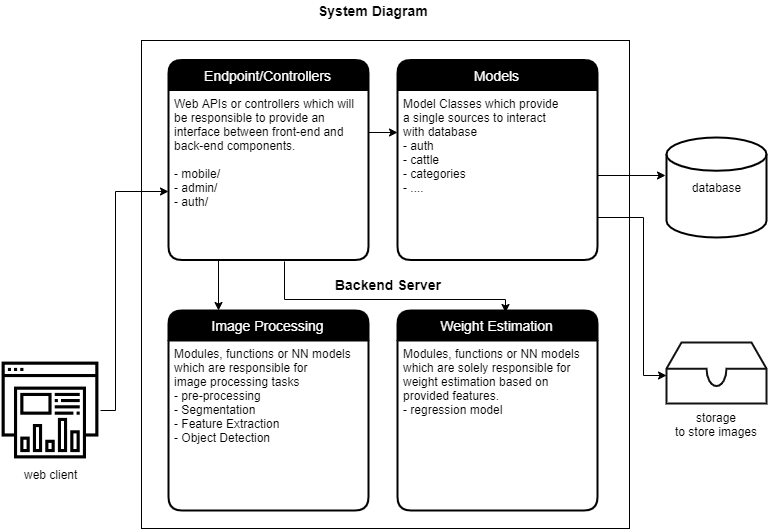
\includegraphics [scale=0.5] {system}
\caption{System Diagram}
\end{figure}


\subsection{Database}
This component will be responsible of storing data into relational format. This will be only accessible by Models (in MVC) component in the back-end. \\  \\
\textbf{Tools and Technologies: } PostgreSQL, SQL.\\

\subsection{Back-end Server}
This component will have further subcomponents:
\begin{enumerate}
\item \textbf{Models:}
This component is responsible to defining the schema of the database and interact with the database. This is the only module which interacts with the database, so that there is one source of truth for insertion and retrival of data. 
\item  \textbf{Image Processing module:}
This component will have methods responsible for segmentation, object detection and features extraction. 
\item \textbf{Weight Estimation:}
		Modules, functions or NN models which are solely responsible for weight estimation based on provided features. 		\\ i.e. regression model

\item \textbf{Endpoints / controllers:}
These Endpoints will define communication routes between server and clients and will bridge between the frontend and backend components. \\
\end{enumerate}
Collectively we refer to \textbf{Image Processing} and \textbf{Weight Estimation} as  \textbf{Core}. \\ \\
\textbf{Tools/Technologies:} OpenCV, Django 2, MXnet, \\

\subsection{Webclient}
 This component will be helping in managing the information of animal and keeping tack of their weights on the go. \\
\textbf{Tools/Technologies:}
 Html, CSS, JavaScript


\pagebreak
\section{Architecture Diagram}

The following is the architecture diagram of the system which would be consists of four different layers. Since the system follow the MVC structure, these layers would be of view, controller, and model layers. There would be another layer of storage, which consists of database of the system. Layers are in hierarchical order, it means that every layer can communicate with its neighbour only. 


\begin{figure}[h]
\centering
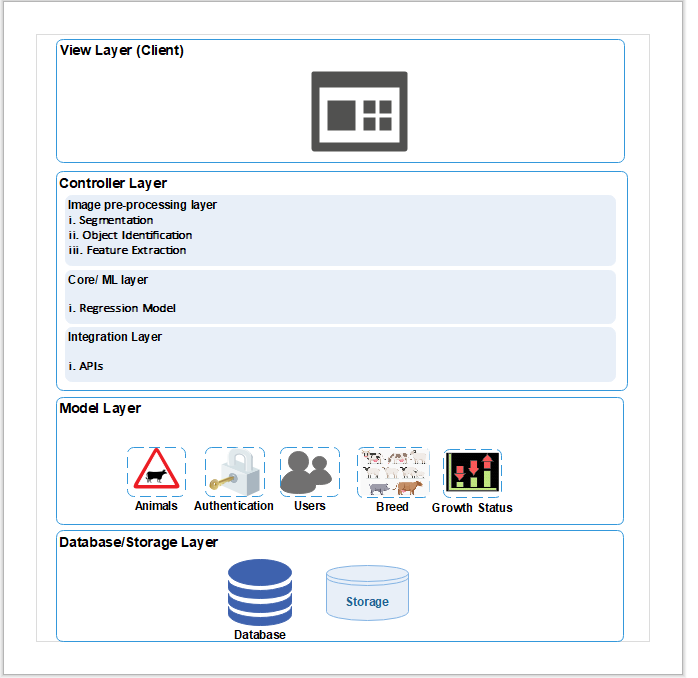
\includegraphics [scale=0.5] {ad.jpg}
\caption{Architecture Diagram}
\end{figure}


\pagebreak 
\section{Use Cases}

This section presents detailed use cases of our system.This diagram illustrates the basic breakdown of our system in terms of use cases and actors. The expanded use cases are provided ahead. 
\begin{figure}[h]
\centering
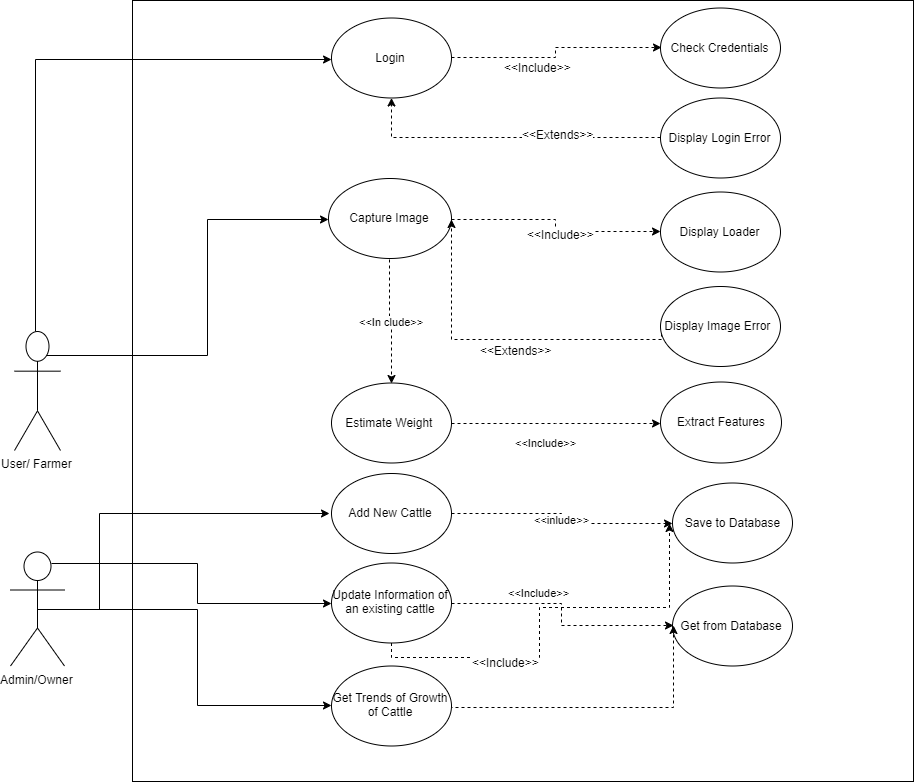
\includegraphics [scale=0.4] {uc}
\caption{Use Case Diagram}
\end{figure}



\pagebreak

\textbf{Use Case 1: Login}

\begin{tabular}{|l|p{.60\textwidth}|p{0.30\textwidth}|}
	\hline
	Use-Case Name: & Login\\ \hline
	Use-Case ID:& UC-01 \\\hline
	Priority:& High\\ \hline
	Source:& None \\ \hline
	Primary Business Actor: & User/Client\\ \hline
	Other Participating Actors:&  No one\\ \hline
	Description:&  The user would login the application as well as admin panel to use the system. Only authenticated users will be allowed to login. \\ \hline
	Precondition:&  User must be registered. \\ \hline
	Trigger:&  When user enters his credentials and clicks on submit. \\ \hline 
	Typical course of events:&  \textbf{Actor Action:}
	\begin{enumerate}
		\item 	User enters the credentials and clicks on submit button.
	\end{enumerate}

	\vspace{2mm}
	
	\textbf{System Action: }
	\begin{enumerate}
		\item System checks the credentials of the user and validate them.
		\item 	If the credentials are valid. User is allowed to use the system, else error generated. 
	\end{enumerate}
	\\ \hline
	Conclusion:  & If credentials are valid, them user will logged in.\\ \hline
	Post Condition: & None \\ \hline
\end{tabular}\\
\\


\pagebreak

\textbf{Use Case 2: Capture Images}

\begin{tabular}{|l|p{.60\textwidth}|p{0.15\textwidth}|}
	\hline
	Use-Case Name: & Capture Images\\ \hline
	Use-Case ID:& UC-02 \\\hline
	Priority:& High\\ \hline
	Source:& None \\ \hline
	Primary Business Actor: & User/Client\\ \hline
	Other Participating Actors:&  No one\\ \hline
	Description:&  The user would capture the image of a cattle from front and side view. The images would be captured from a particular angle and only two images would be captured. \\ \hline
	Precondition:&  User must be authenticated. \\ \hline
	Trigger:&  When user is logged in into the system and click on the camera button to capture the image.  \\ \hline 
	Typical course of events:&  \textbf{Actor Action:}
	\begin{enumerate}
		\item The actor clicks on the button to capture image. 
		
	\end{enumerate}
	\vspace{2mm}
	
	\textbf{System Action: }
	\begin{enumerate}
		\item	After capturing the image, the image is sent to server for further processing.  
		
	\end{enumerate}
	\\ \hline
	Conclusion:  & The image is captured by the mobile application at a certain angle and sent to server for further processing. \\ \hline
	Post Condition: & The image is sent to the server  for further processing.  \\ \hline
\end{tabular}\\


\pagebreak

\textbf{Use Case 3: Add New Cattle}\\


\begin{tabular}{|l|p{.60\textwidth}|p{0.15\textwidth}|}
	\hline
	Use-Case Name: & Add New Cattle\\ \hline
	Use-Case ID:& UC-05 \\\hline
	Priority:& High\\ \hline
	Source:& None \\ \hline
	Primary Business Actor: & Farm's owner/ Admin.\\ \hline
	Other Participating Actors:&  System/Admin Panel\\ \hline
	Description:& When new cattle is added in the farm, the basic details of the cattle such as age, gender, unique id is stored in the system’s database through admin panel \\ \hline
	Precondition:& User must be authenticated.   \\ \hline
	Trigger:& On clicking the “Add new cattle” button on admin panel.    \\ \hline 
	Typical course of events:&  \textbf{Actor Action:}
	\begin{enumerate}
		\item Admin click on “Add new cattle” tab and enters the information related to animal and click on the save button.  
	\end{enumerate}
	\textbf{System Action: }
	\begin{enumerate}
		\item 	System take those information and send it to database to save. 
	\end{enumerate}
	
	\\ \hline
	Conclusion:  & The record of the new cattle is saved into the database. \\ \hline
	Post Condition: &The information can be shown through admin panel.  \\ \hline
\end{tabular}\\


\pagebreak
\textbf{Use Case 4: Update Cattle Information into the Database}\\


\begin{tabular}{|l|p{.60\textwidth}|p{0.15\textwidth}|}
	\hline
	Use-Case Name: & Update cattle information into the database. \\ \hline
	Use-Case ID:& UC-06 \\\hline
	Priority:& High\\ \hline
	Source:& None \\ \hline
	Primary Business Actor: & Farm's owner/ Admin.\\ \hline
	Other Participating Actors:&  System/Admin Panel\\ \hline
	Description:& The cattle information can be updated by admin at any time when needed. The updated information will overwrite the previous information.  \\ \hline
	Precondition:& The cattle information is already added and saved in the system.    \\ \hline
	Trigger:& When information changes, the admin will update the information into the system.    \\ \hline 
	Typical course of events:&  \textbf{Actor Action:}
	\begin{enumerate}
		\item Admin click on “Update cattle info” tab and updates the information click on the save button.  
	\end{enumerate}
	\textbf{System Action: }
	\begin{enumerate}
		\item The system save the updated information into the database.
	\end{enumerate}
	
	\\ \hline
	Conclusion:  & The information is updated into the database.\\ \hline
	Post Condition: &The updated information is displayed through admin panel. \\ \hline
\end{tabular}\\


\pagebreak
\textbf{Use Case 5: Get Trends of Growth of Cattle}\\


\begin{tabular}{|l|p{.60\textwidth}|p{0.15\textwidth}|}
	\hline
	Use-Case Name: & Get trend of growth of cattle. \\ \hline
	Use-Case ID:& UC-07 \\\hline
	Priority:& High\\ \hline
	Source:& None \\ \hline
	Primary Business Actor: & Farm's owner/ Admin.\\ \hline
	Other Participating Actors:&  System/Admin Panel\\ \hline
	Description:& The cattle growth trend will be shown on admin panel on the basis of their weight estimated by the system. The trends will be shown on individual level. The pi-chart would also be displayed on panel to show the overall progress.  The system will display the last six months record.   \\ \hline
	Precondition:& The cattle information is already added and saved in the system.     \\ \hline
	Trigger:&It would be the core functionality of the admin panel and will be displayed by default on admin panel.     \\ \hline 
	Typical course of events:&  \textbf{Actor Action:}
	\begin{enumerate}
		\item No action would be done by user.  
	\end{enumerate}
	\textbf{System Action: }
	\begin{enumerate}
		\item The system will display the trends to show the growth progress. 
	\end{enumerate}
	
	\\ \hline
	Conclusion:  & The growth trends will be shown on the panel.\\ \hline
	Post Condition: &  The user can keep track of the animal’s weight of last six month. \\ \hline
\end{tabular}\\


\chapter{Software Design Specification (SDS)}
\label{chap:sds}

This chapter provides important artifacts related to design of our project.

\section{Software Design}

This section presents the UML class diagram and gives a brief description of each class in our system. Attributes and methods of each class and relationship among classes are clearly presented. Our project contains the following classes. All the following classes except for Static classes are derived from Django Model Class because they will be directly communicating to database and define schema of it.


\begin{figure}[h]
\centering
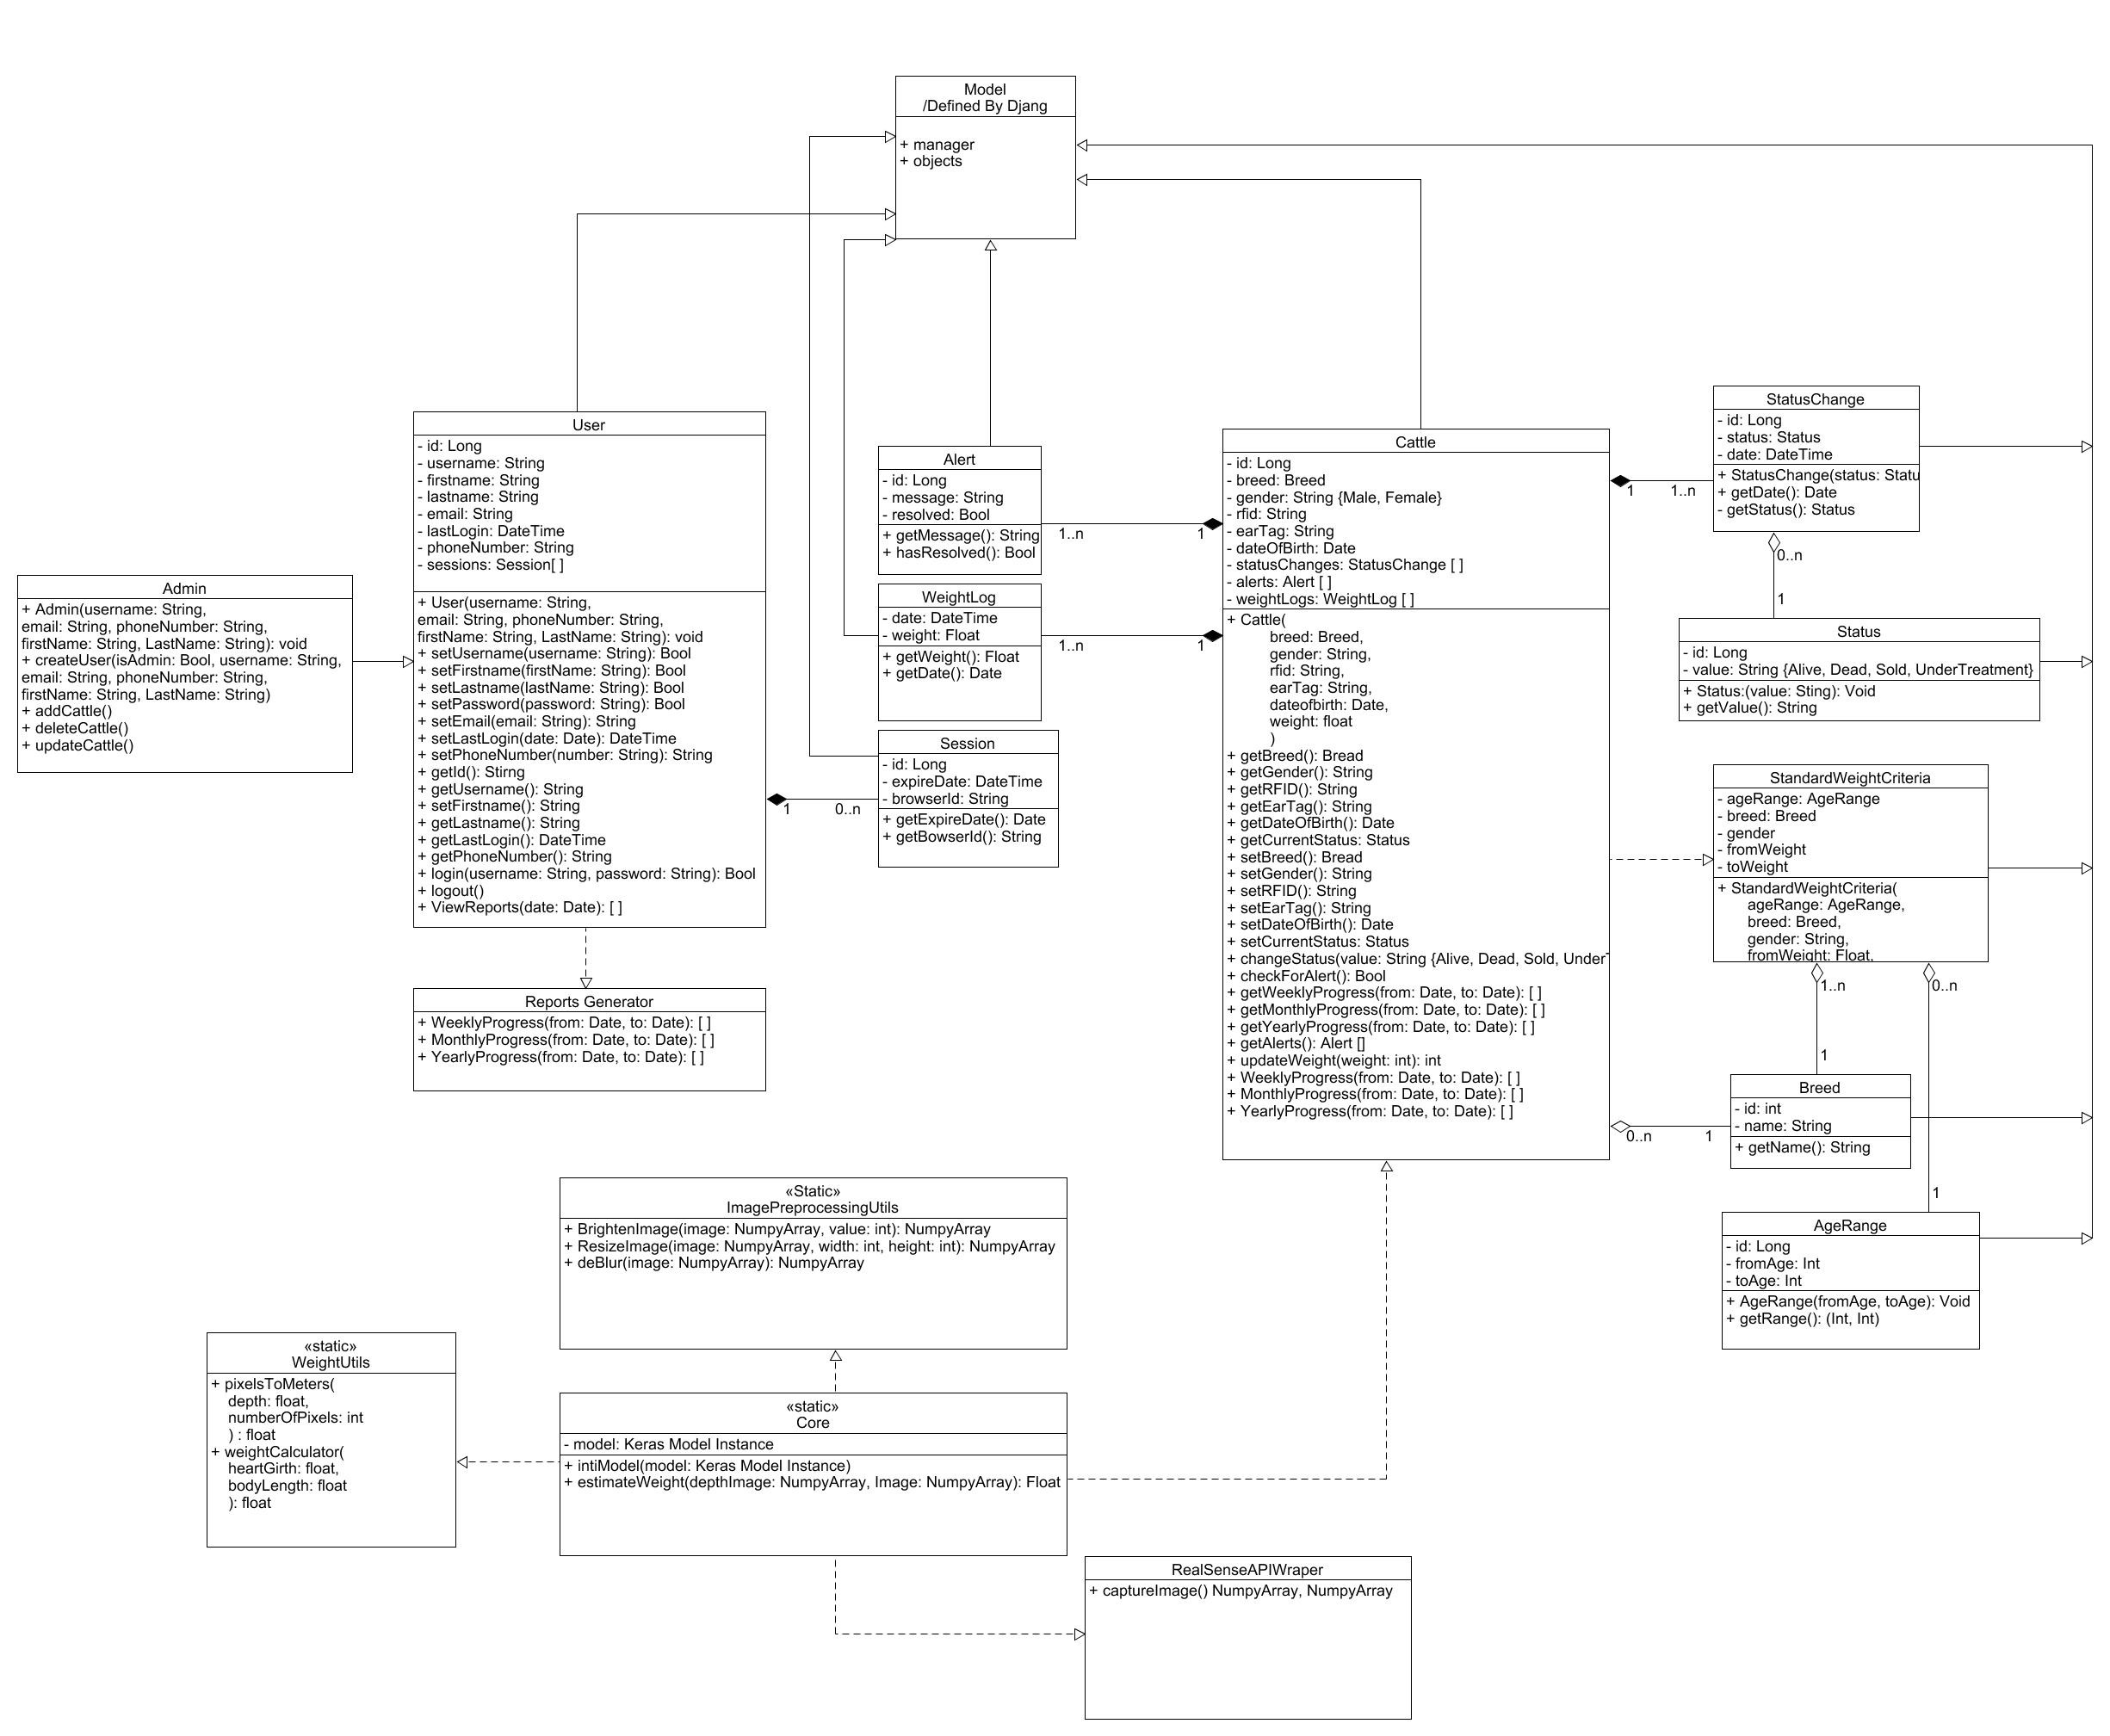
\includegraphics [scale=0.2] {FYP_UML}
\caption{Software Design Diagram (Class Diagram)}
\end{figure}


\subsection{User}
This class represents a generic user in out system. In the system there are two types of user \textbf{Admin} and \textbf{Simple User} therefore another class '\textbf{Admin}' is derived from this class. 

The class encapsulates information like \textbf{firstname, lastname, username, password, currently active session} for a perticular instance of a user.

\subsection{Admin}

This is a subclass of user which has additional access of \textbf{creating}, \textbf{updating} and deleting a users also, only the admin has access to \textbf{CRUD} operations on \textbf{Cattle}.

\subsection{Sessions}

Session encapsulates the information about a particular session of a user. User has an array of his/her currently active sessions. 

\subsection{Cattle}
This class encapsulates all details of a cattle object. some of the attributes are \textbf{rfid, earTag, dateOfBirth}. Since cattle must belong to a specific \textbf{Breed}, it store reference to the breed it belongs to. It also has some object level and some class level methods to access reports. All class methods are capitalized. While generating alerts for a cattle it is dependent on standard weight criteria.  

\subsection{Alert}
This class encapsulates details of an alert object. An alert will be generated if cattle is exceeding its \textbf{Standard Weight Criteria}.  

\subsection{Standard Weight Criteria}
This class encapsulates information about a weight criteria for a specific breed for a specific age range. 

\subsection{Age Range:}
This class encapsulates information about an age range. An Age range is a range of age which is required to define a standard weight criteria.

\subsection{Breed:}
The class encapsulates information about a breed. 

\subsection{Status}
The class encapsulates information about a Status of a cattle. Status specifies whether the cattle is under overweight, underweight, good or bad condition.

\subsection{Status Change}
This class encapsulates change in the state of a cattle at a particular instance. A Cattle object has an array of status changes in it. 

\subsection{Weight Log}
This class encapsulates information about weight change of a particular cattle object at a particular instance. A Cattle object has an array of Weight Logs in it. 

\subsection{Core (Static Class)}
This class has some static methods for weight estimation and model initiation. the classes is dependent on the static methods of other three static classes of \textbf{WeightUtils, IntelRealsenseAPIWraper, and ImagePreprocessingUtils} .


\section{Data Design}

This section presents the structure of our database that caters to persistent data storage in our project. The structure is shown as a normalized data model for relational databases. It clearly shows entities, attributes, relationships with their cardinalities, and primary and foreign keys. We have used DB designer (or any other similar data modeling tool) to build our data model.


\begin{figure}[h]
\centering
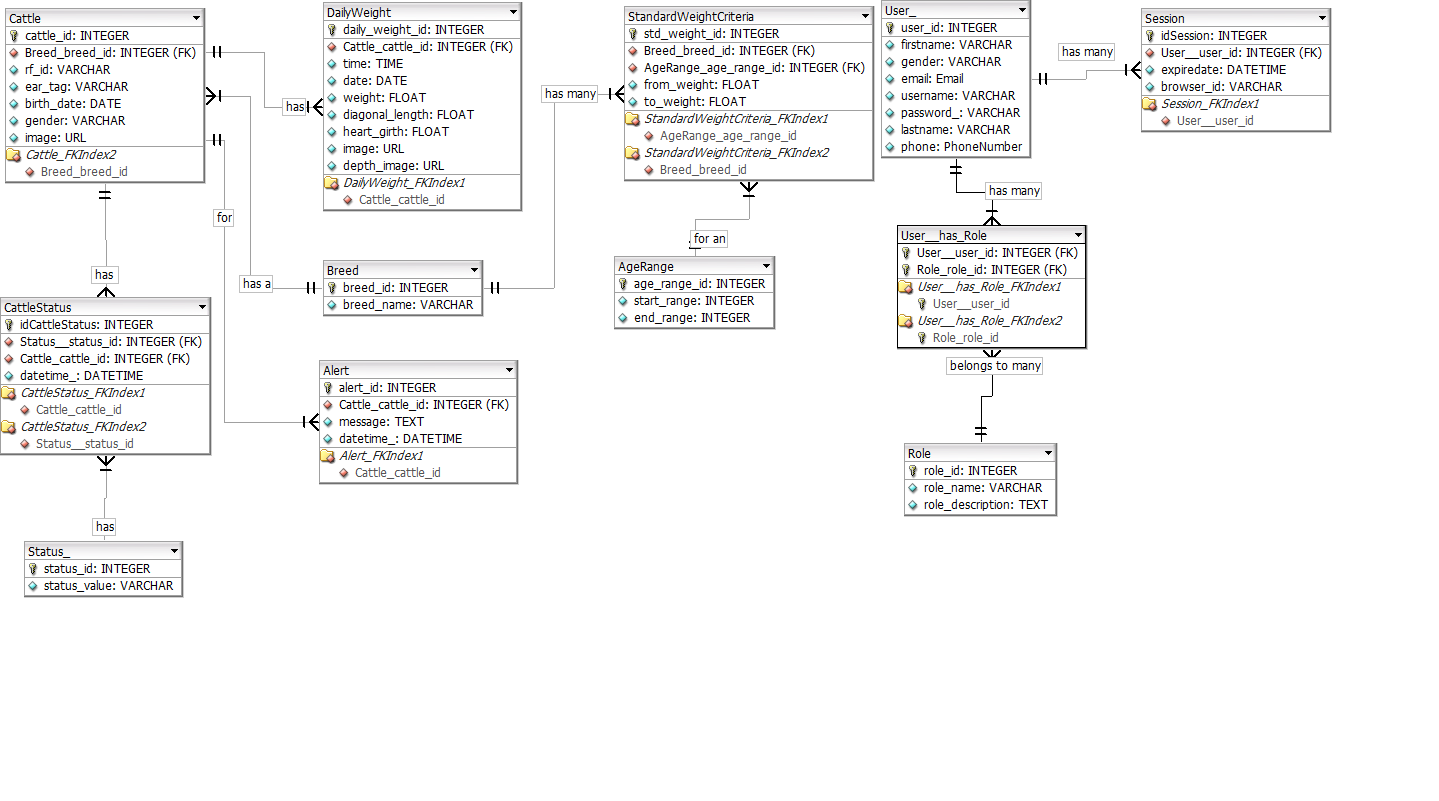
\includegraphics [scale=0.3] {erd.png}
\caption{Entity Relationship Diagram}
\end{figure}

The system has following Entities:
\subsection{User}
This represents a generic user and its attributes. 

\subsection{Session}
This represent a serverside session of a user. User and Session have a one to many relationship therefore userId is stored as foreign key in  Session. 

\subsection{Role }
Role is a generic role representation in database. User and Roles have many to many relationship therefore a middle entity \textbf{UserHasRole} is use to resolve this.

\subsection{Cattle}
This entity represents a Cattle's attributes which are stored in database.  A cattle must have a \textbf{Breed} therefore it stores BreedId as a foreign key.

\subsection{Breed}
The entity represents a breed in database. Since a breed can belong to many cattle its id is stored as foreign key in cattle's table. A breed can also have a different weight criteria based on gender and age range therefore its id is stored as foreign key in \textbf{StandardWeightCriteria} .

\subsection{Alert}
Alert are generated when an animals state is changed. Alert entity shows the attributes stored in database. Since an alert is related to a particular cattle, cattle id is stored as a foreign key in Alert. 

\subsection{Standard Weight Criteria}
Standard weight Criteria is different for each breed and gender. This entity represents its representation in database. It has a one to many relation with breed and AgeRange their ids are stored in this entity. 


\subsection{Age Range:}
An Age range is a range of age which is required to define a standard weight criteria. 

\subsection{Status}
Status specifies whether the cattle is under overweight, underweight, good or bad condition. Its id is stored for each status change for a cattle in Status Change Entity along with Cattle Id.

\subsection{Status Change}
This entity represents change in the state of a cattle at a particular instance. It stores Cattle id and State id in it. 

\subsection{Weight Log}
It represents a weight change of a particular cattle object at a particular instance.




































\chapter{Experiments and Results}
\label{chap:results}
The main component of our system is the "Core Component" which is responsible for estimating the weight of a cattle given an RGB image along with a per-pixel depth map. So, most of the time was spent in in the development of this component. The experiments which we carried out throughout the span of this project can be divided into the following two main categories.
\begin{enumerate}
\item Deep learning Models 
\item Camera and Depth Related Experiments 
\end{enumerate}
\subsection{Deep Learning Models}
Almost \(75\%\) of the time was dedicated to collect data whose description is in 3.5.5 Dataset and Augmentation section, to do experiments, and to come up with a better model. The biggest challenge for this part was the availability of dataset and also weight of the cattle. All dataset, which is used throughout this project, is collected by our team. 
\\

\subsubsection{Experiments on Dataset V1 for Localization}

On dataset V1, we tried to solve our problem as a localization problem through transfer learning. In localization problem we assume that there is only one object in an image which we are trying to detect. This fact give us an advantage that we know exactly how many bounding boxes we have to predict. In this experiment Pre-trained networks VGG16 and Resnet were used as base networks. At the end of these networks we attached our own fully connected network for regression on the features extracted by the base networks. 

Initially, we trained only fully connected layers for two bounding boxes. Then we trained only fully connected layers for one bounding box. We then unfreeze some convolution layers and train them for both two bounding boxes and one bounding box. Global Average Pooling was used for Localization. But we were unable to get the satisfactory results. Our min loss was 4.68 on mean absolute error. 

\begin{figure}[h]
\centering
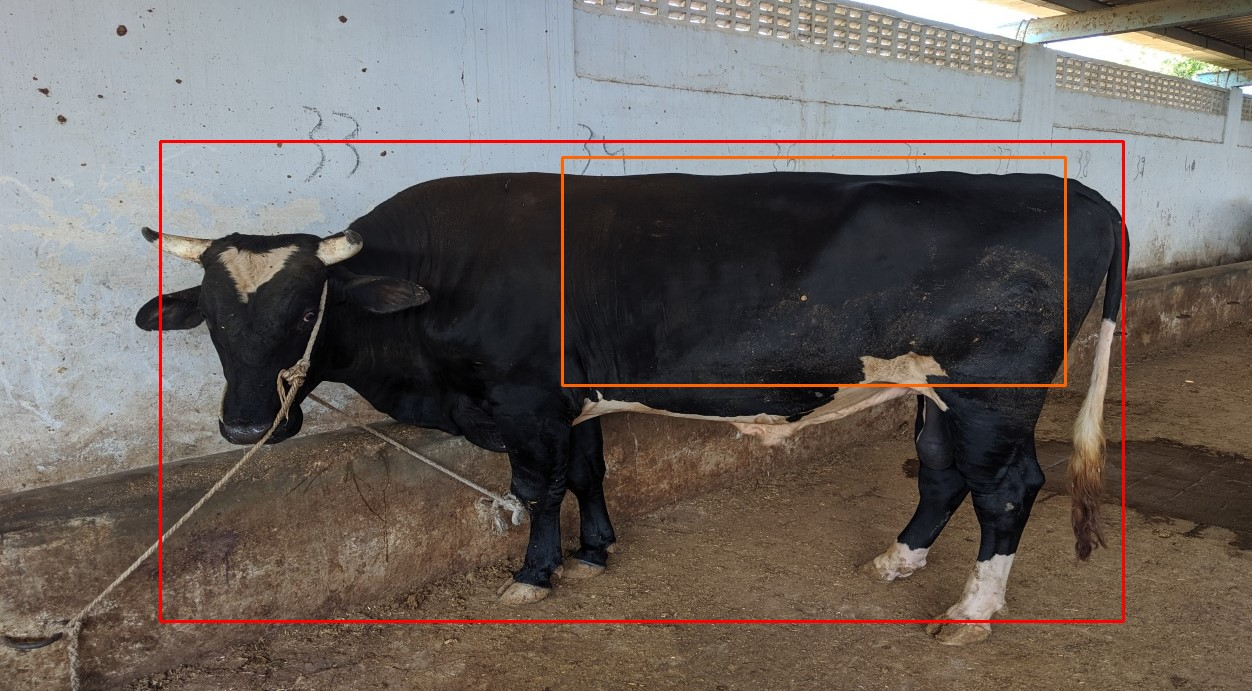
\includegraphics[scale=0.3]{v1-loc.jpg}
\caption{Output of Models for Object Localization trained on V1}
\end{figure}


\begin{figure}[h]
\centering
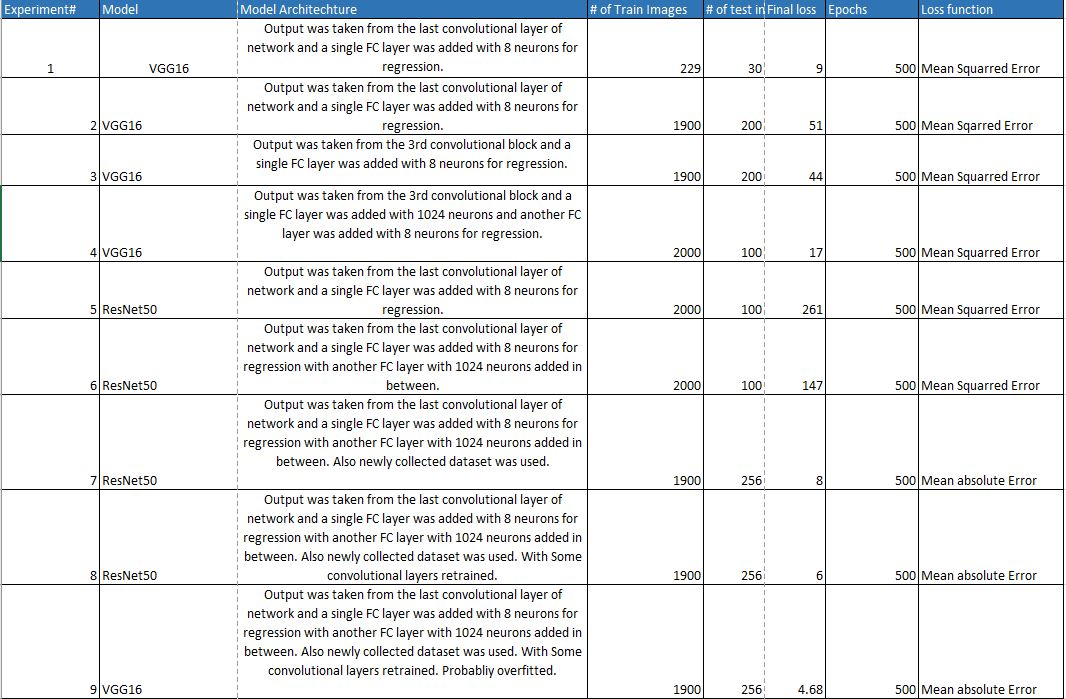
\includegraphics[scale=0.5]{Capture.JPG}
\caption{Results of Models for Object Localization trained on V1}
\end{figure}
\pagebreak



\subsubsection{Experiments on Dataset V2 for Localization}
In this experiment, cattle images were cropped and we tried to predict inner bounding boxes. We assumed that it will learn better features due to the lack of background. However, this did not produce the results we were looking for

The problem we observed in both of the experiments was the over fitting of train data. They seemed to perform good on train data while it performed worse on test data. But in order to make our solution work we needed very tight bounding box. After a lot of effort we then trained Yolo and Mask RCNN. 

\subsubsection{YOLO}
After experimenting with object localization and not getting satisfactory results we turned towards YOLO object detector. YOLO stands for You Only Look Once. The advantages of using YOLO are numerous and one of them is speed, YOLO is the fastest deep learning based object detector which offers reasonable accuracy.
We trained YOLO on Dataset V2 containing 1200 images. After 100 epochs we got loss of 11.54 units on YOLO custom loss function.
On the test set we acheived an average IoU of \(80\%\).
The bounding box detected by YOLO trained on dataset V2 is shown below.\\
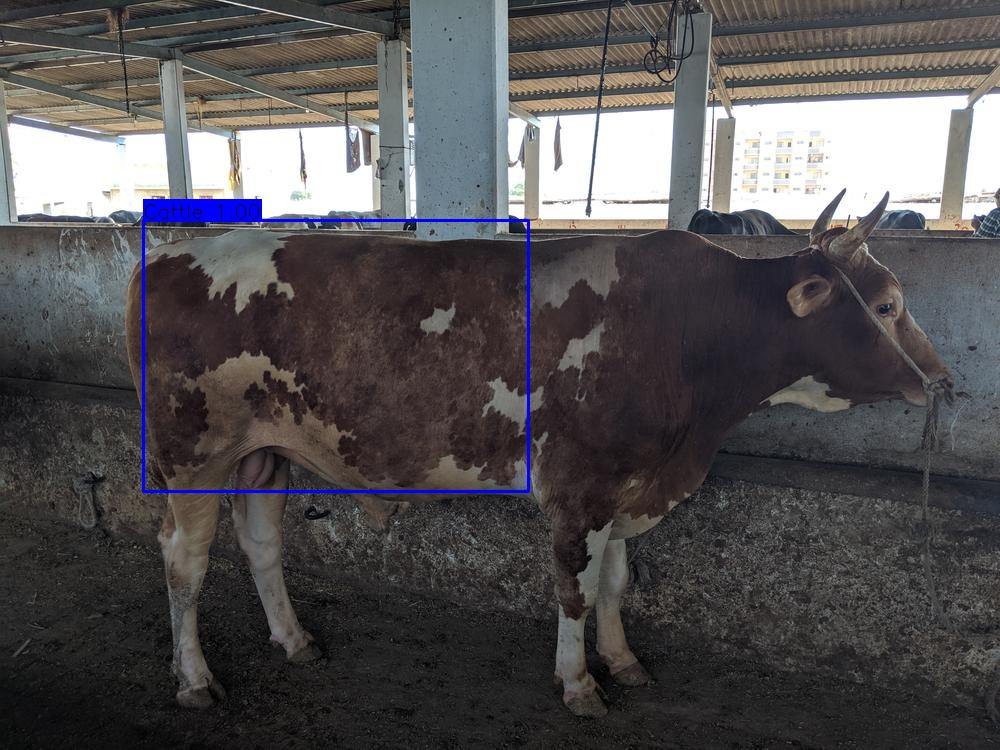
\includegraphics[scale = 0.2]{images/result.jpg}

The results from YOLO may look reasonable but they could be made better with little adjustment. Or we can collect a bigger dataset and train YOLO on it better performance in terms of detection accuracy. In an ideal case there should not be a single pixel on the box that is outside cattle body.

\subsubsection{Mask R-CNN}

In our quest for a perfect weight estimater we also explored Mask R-CNN to get a better more robust system. The idea was to segment out the cattle from the RGB image. Then superimpose the cattle mask on the depth channel. Essentially, the extracting all the depths the lies on the cattle. We then input the depth values to an Artificial Neural Network (ANN) and frame the problem as regression problem. The problem with this approach is that it needs weight labels for each cattle in the dataset, which is not available. Nevertheless we went on to explore this approach as weight labels can be collected later.\\

We trained a Mask-RCNN on Dataset V2 and got the following results.\\
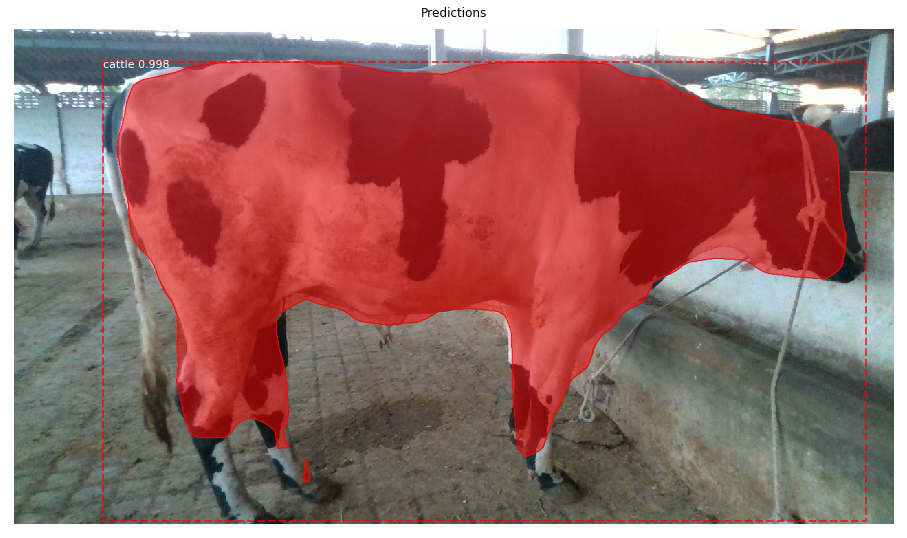
\includegraphics[scale=0.3]{images/1122.png}\\


But we can not proceed any further with this approach to make an actual weight estimator as we dont have weight labels of each cattle. But what we can do is prove that the ANN which we are going to train once we get the weight labels will work, by calculating the proxy Factor in the next sub heading.

\subsubsection{Factor}


\subsection{Camera and Depth Related Experiments}
The purpose of our deep learning models to get the rectangle so that we can take out the pixels' vector which lies on the heart girth of the cattle once we have this vector we have to get the real world measurement of the heat girth of the cattle. 


\subsubsection{Curve Length Estimation:}

In the above mentioned approaches the final result we get is a bounding box encapsulating the information of body length in the diagonal and heart girth measurements in height of the box. Since these values are just only represented by two pixel coordinates top-left and bottom right. As mentioned earlier to get the measurements accurate we have to incorporate the depth information. Since we have depth map and RGB image of same dimensions and from same camera we can safely map this bounding box to depth image as well. 

Once we have a this image box on depth image we will extract out the vector of pixels from the heart girth line of the bounding box and diagonal vector from pixels starting from bottom left and the top right  point in this image.
Once we have these two vectors we can convert it into real world measurements using the procedure defined below.   
For the simplicity forget the consider that we have a formula which converts  given number of pixels into meters and also take a distance from camera to take care of the scaling, because otherwise far objects appear small in image. now given this formula consider the abdomen of the cattle. It is mostly symmetric from both sides. If we take the measurements of a heart girth and body length curves on the surface of the abdomen, which is like a semi-ellipse from one side, will have huge factor in measurements. So to preserve this information we will use the mathematical approach, discussed in Appendix A, to get the length of heart girth circumference and body length more accurately. 






 

 


\chapter{Conclusion and Future Work}
\label{chap:outro}
If we look at the progress of this project so we were able to develop the Admin Panel success fully and sub programs to estimate the weight given depth vectors were also developed. The only part where we still struggled was the ``Core Component". Our dataset collection was impacted due to Covid-19. The best we have now is YOLO object detector which is giving us on average \(80\%\) workable predictions, it gives us the bounding box for abdomen which we use to extract heart girth's information . Since we also have proposed that we can segment out the mask of cattle from Mask RCNN, which we trained on our own, because existing one was not as accurate as we wanted on cattle's side view, and extract depth information corresponding to this mask from image then given this information if we have cattle's weight labeled dataset we can train a regression model on this depth mask to get the accuracy up to \(90-95\%\) because the depth values encapsulate the whole 3D information about the cattle. This is the future work we propose for which Mask RCNN is trained for better masks for this problem. Also we have compiled a very diverse dataset for this problem which we think is going to help a lot if someone tries to solve this problem in future. 


\begin{appendices}

\titleformat{\chapter}[hang]{\bf\huge}{Appendix \thechapter.}{2pc}{}
% \titleformat{\chapter}[hang]{\bf\huge}{\thechapter.}{2pc}{}

  
% This appendix is optional.
\chapter{More Math}
\begin{figure}[h]
\centering
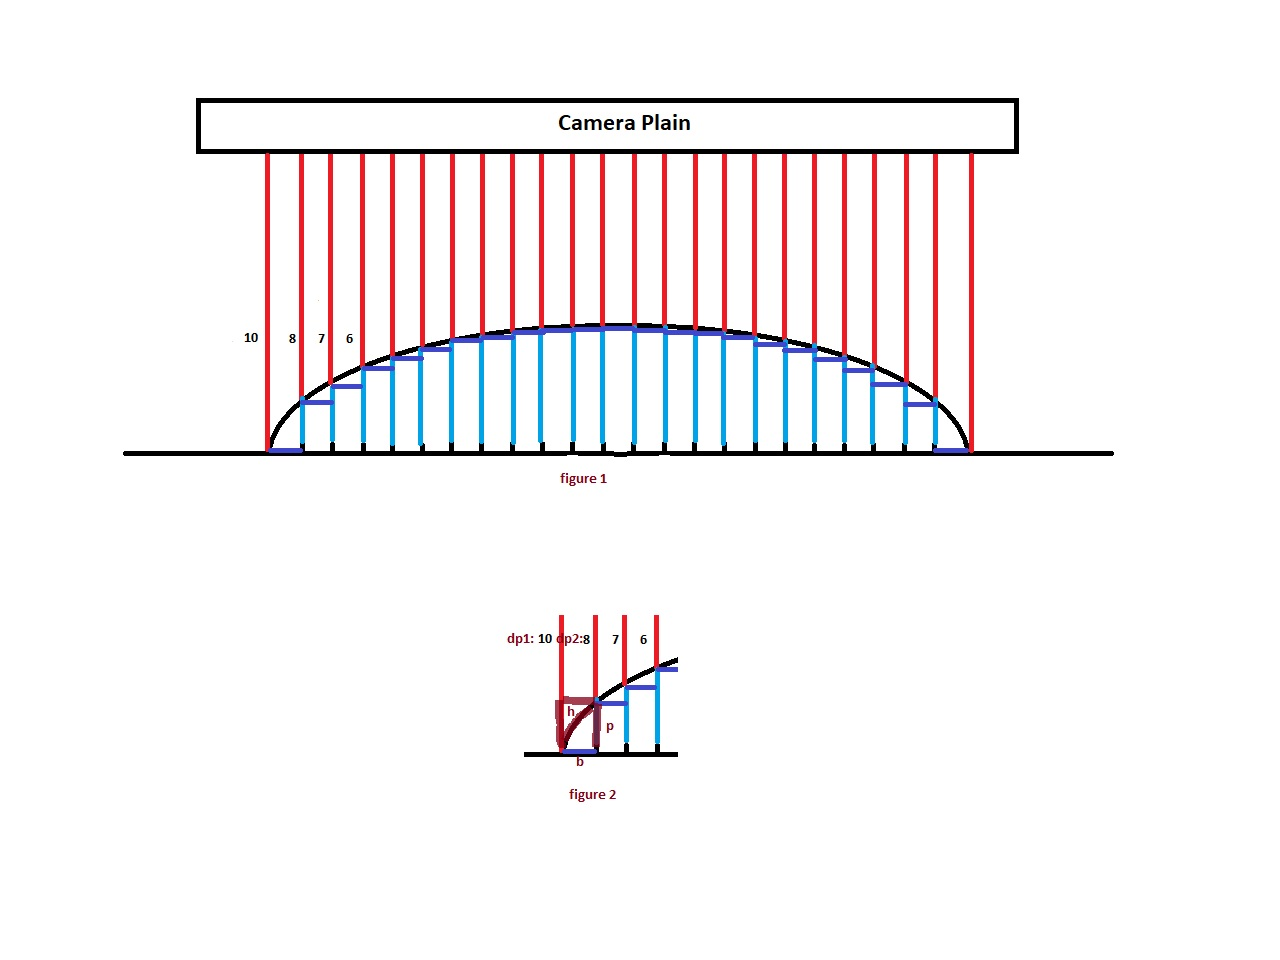
\includegraphics[scale=0.5]{depthToPixels.jpg}
\caption{Heart girth measurement approach}
\end{figure}

Consider figure A.1. Here picture of a surface is taken from a dept camera. Black curve represents the surface and the red lines represent per-pixel distance from camera. Since we assumed that we have a function which can convert number of pixels covered at certain depth to meters, we can get the measures for each pixel in meters. But our problem is to get the length of the length of the curve in meters while preserving the curve, we break the curve into small segments each segment is break after one pixel. If we have to estimate the curve of this segment we can do  so by fitting a triangle on it.  Where base of the triangle is \\ 
\begin{center}
 maxpoint = argmax(depth of P1, depth of P2)  
$b$ = pixelToReal (depth = maxpoint, numberofpixels = 1 ) 
 
\end{center}
Now we have the base in meters we have to calculate the perpendicular or the height this is simply the absolute difference between the depth of P1 and P2 
\begin{center}
 $p$ = \(|depth of P1 -  depth of P2|\) 

\end{center}

once we have the the base and perpendicular we can use the Pythagoras theorem to calculate the hypotenuse or the length of the segment  
\begin{center}

$h=\sqrt{ p^2 + b^2}$ 

\end{center}
						
now we have the formula we can apply this over all segments sum the all segments' length to estimate the length of the curvature. hence by using this technique we can get the the length of heart girth circumference and body length more accurately.


% This appendix is required if the data set is not fully described in the main text.
\chapter{Data}
\textbf{The complete dataset our project can be found at \href{https://drive.google.com/drive/folders/1-NH5rOB6CmhRUDG_SNe7LSXv1LgAC3d2?usp=sharing}{this Google Drive link}.}




% This appendix is required if the code is not fully described in the main text.
\chapter{Code}
Here is the part of our code. This code is to capture the images of cattle and to collect dataset. The camera would be connected to laptop and this script would run to capture the cattle images. This would take two paths as parameters to save RGB and depth images and also image number of the captured image. 
\newline

% inspired by https://xkcd.com/221/
\lstinputlisting[language=Python,showstringspaces=false]{code/capture.py}

% Alternately...

\textbf{The complete code of our project can be found at \href{https://github.com/am02464/InstaWeight}{this GitHub link}.}
%%% Local Variables:
%%% mode: latex
%%% TeX-master: "../report"
%%% End:

\end{appendices}

\chapter{References}
\label{chap:references}
\begin{enumerate}
	\item Siregar,S. B.,2007. Fattening Cattle. Jakarta : Penebar Swadaya.
	\item Soeprapto,H., Z.Abidin. 2006. How Fattening Beef Cattle. Jakarta : Agromedia Press
	\item  M. D. Deddy B. Lasfeto, "A measuring weight model of timor's beef cattle based on image," International Journal of Engineering and Technology (IJET), p. 12. 
	\item T. M. Banhazi, "Weight Estimation Using Image Analysis and Statistical Modelling: A Preliminary Study," Applied engineering in agriculture, 2007.
	\item Mehrotra, R., and S. Zhan. 1996. A computational approach to zero-crossing-based two-dimensional edge detection. Graphical Models and Image Processing 58(1): 1-17.
	\item Z. H. Pradana, B. H. and S. D., "Beef Cattle Weight Determine By Using Digital Image Processing," The 2016 International Conference on Control, Electronics, Renewable Energy and Communications (ICCEREC), 2016.
	\item A. Yamashita, "Estimation of Calf Weight from Fixed-Point Stereo Camera Images Using Three Dimensional Successive Cylindrical Model," Proceedings of the 5th IIAE International Conference on Intelligent Systems and Image Processing 2017, 2017.
	\item Zhou, B. (n.d.). Learning Deep Features for Discriminative Localization. Retrieved from \url{http://cnnlocalization.csail.mit.edu/Zhou_Learning_Deep_Features_CVPR_2016_paper.pdf}


	\item R. Dalai and K. K. S. , "Weight Estimation through Image Analysis," International Journal of Computer Trends and Technology (IJCTT), vol. 49, pp. 1-5, July 2017.
\end{enumerate}

\chapter{Vita}
\label{chap:vita}

\begin{center}
    Sayyda Sahar Fatima
\end{center}
Sayyda Sahar Fatima is graduated from Habib University in 2020, with a degree in Bachelor of Computer Science. She is Top Performer student and has received Dean's List award multiple times. She is very focused and punctual and does her work with full concentration. She enjoys her work and tries to explore innovative things and technologies. Furthermore, she has experienced in the field of web development and has worked as a software developer at WeUno. 


\begin{center}
    Atif Mehmood
\end{center}
Atif Mehmood is one of the hard working graduate of Habib University Class of 2020. He is a quick learner and is always excited about solving new problems and learning something new. He has a particular interest in Software Development and Computer Vision. He has worked at Afiniti and currently working as a Software Engineer for Stellic on their reimagined platform for degree planning, advising and auditing. 

\begin{center}
    Mohammad Ateeb Ahmed
\end{center}
Mohammad Ateeb Ahmed is a computer science graduate of Habib University, really excited about theoretical computer science and physics. He is more interested in doing research work and tries to solve the a problem by applying different algorithms and problem solving techniques. 


% Print the bibliography with a ToC entry and titled, "References".
\printbibliography[heading=bibintoc,title={References}]

\end{document}

%%% Local Variables:
%%% mode: latex
%%% TeX-master: t
%%% End:
